%% bare_conf.tex
%% V1.3
%% 2007/01/11
%% by Michael Shell
%% See:
%% http://www.michaelshell.org/
%% for current contact information.
%%
%% This is a skeleton file demonstrating the use of IEEEtran.cls
%% (requires IEEEtran.cls version 1.7 or later) with an IEEE conference paper.
%%
%% Support sites:
%% http://www.michaelshell.org/tex/ieeetran/
%% http://www.ctan.org/tex-archive/macros/latex/contrib/IEEEtran/
%% and
%% http://www.ieee.org/

%%*************************************************************************
%% Legal Notice:
%% This code is offered as-is without any warranty either expressed or
%% implied; without even the implied warranty of MERCHANTABILITY or
%% FITNESS FOR A PARTICULAR PURPOSE!
%% User assumes all risk.
%% In no event shall IEEE or any contributor to this code be liable for
%% any damages or losses, including, but not limited to, incidental,
%% consequential, or any other damages, resulting from the use or misuse
%% of any information contained here.
%%
%% All comments are the opinions of their respective authors and are not
%% necessarily endorsed by the IEEE.
%%
%% This work is distributed under the LaTeX Project Public License (LPPL)
%% ( http://www.latex-project.org/ ) version 1.3, and may be freely used,
%% distributed and modified. A copy of the LPPL, version 1.3, is included
%% in the base LaTeX documentation of all distributions of LaTeX released
%% 2003/12/01 or later.
%% Retain all contribution notices and credits.
%% ** Modified files should be clearly indicated as such, including  **
%% ** renaming them and changing author support contact information. **
%%
%% File list of work: IEEEtran.cls, IEEEtran_HOWTO.pdf, bare_adv.tex,
%%                    bare_conf.tex, bare_jrnl.tex, bare_jrnl_compsoc.tex
%%*************************************************************************

% *** Authors should verify (and, if needed, correct) their LaTeX system  ***
% *** with the testflow diagnostic prior to trusting their LaTeX platform ***
% *** with production work. IEEE's font choices can trigger bugs that do  ***
% *** not appear when using other class files.                            ***
% The testflow support page is at:
% http://www.michaelshell.org/tex/testflow/



% Note that the a4paper option is mainly intended so that authors in
% countries using A4 can easily print to A4 and see how their papers will
% look in print - the typesetting of the document will not typically be
% affected with changes in paper size (but the bottom and side margins will).
% Use the testflow package mentioned above to verify correct handling of
% both paper sizes by the user's LaTeX system.
%
% Also note that the "draftcls" or "draftclsnofoot", not "draft", option
% should be used if it is desired that the figures are to be displayed in
% draft mode.
%
\documentclass[conference]{IEEEtran}
% Add the compsoc option for Computer Society conferences.
%
% If IEEEtran.cls has not been installed into the LaTeX system files,
% manually specify the path to it like:
% \documentclass[conference]{../sty/IEEEtran}

\usepackage{times,amsmath,epsfig}
\usepackage[linesnumbered,ruled]{algorithm2e}

%\usepackage[pdftex]{graphicx}
% For figures
\usepackage{graphicx} % more modern
\usepackage{epsfig} % less modern
\usepackage{subfigure}
\usepackage{enumerate}
%\usepackage[pdftex]{graphicx}
% For figures
\usepackage{graphicx} % more modern
%\usepackage{epsfig} % less modern
\usepackage{subfigure}

\usepackage{mathrsfs}
\usepackage{amsmath}
\usepackage{epstopdf}


% Some very useful LaTeX packages include:
% (uncomment the ones you want to load)


% *** MISC UTILITY PACKAGES ***
%
%\usepackage{ifpdf}
% Heiko Oberdiek's ifpdf.sty is very useful if you need conditional
% compilation based on whether the output is pdf or dvi.
% usage:
% \ifpdf
%   % pdf code
% \else
%   % dvi code
% \fi
% The latest version of ifpdf.sty can be obtained from:
% http://www.ctan.org/tex-archive/macros/latex/contrib/oberdiek/
% Also, note that IEEEtran.cls V1.7 and later provides a builtin
% \ifCLASSINFOpdf conditional that works the same way.
% When switching from latex to pdflatex and vice-versa, the compiler may
% have to be run twice to clear warning/error messages.






% *** CITATION PACKAGES ***
%
%\usepackage{cite}
% cite.sty was written by Donald Arseneau
% V1.6 and later of IEEEtran pre-defines the format of the cite.sty package
% \cite{} output to follow that of IEEE. Loading the cite package will
% result in citation numbers being automatically sorted and properly
% "compressed/ranged". e.g., [1], [9], [2], [7], [5], [6] without using
% cite.sty will become [1], [2], [5]--[7], [9] using cite.sty. cite.sty's
% \cite will automatically add leading space, if needed. Use cite.sty's
% noadjust option (cite.sty V3.8 and later) if you want to turn this off.
% cite.sty is already installed on most LaTeX systems. Be sure and use
% version 4.0 (2003-05-27) and later if using hyperref.sty. cite.sty does
% not currently provide for hyperlinked citations.
% The latest version can be obtained at:
% http://www.ctan.org/tex-archive/macros/latex/contrib/cite/
% The documentation is contained in the cite.sty file itself.






% *** GRAPHICS RELATED PACKAGES ***
%
\ifCLASSINFOpdf
  % \usepackage[pdftex]{graphicx}
  % declare the path(s) where your graphic files are
  % \graphicspath{{../pdf/}{../jpeg/}}
  % and their extensions so you won't have to specify these with
  % every instance of \includegraphics
  % \DeclareGraphicsExtensions{.pdf,.jpeg,.png}
\else
  % or other class option (dvipsone, dvipdf, if not using dvips). graphicx
  % will default to the driver specified in the system graphics.cfg if no
  % driver is specified.
  % \usepackage[dvips]{graphicx}
  % declare the path(s) where your graphic files are
  % \graphicspath{{../eps/}}
  % and their extensions so you won't have to specify these with
  % every instance of \includegraphics
  % \DeclareGraphicsExtensions{ }
\fi
% graphicx was written by David Carlisle and Sebastian Rahtz. It is
% required if you want graphics, photos, etc. graphicx.sty is already
% installed on most LaTeX systems. The latest version and documentation can
% be obtained at:
% http://www.ctan.org/tex-archive/macros/latex/required/graphics/
% Another good source of documentation is "Using Imported Graphics in
% LaTeX2e" by Keith Reckdahl which can be found as epslatex.ps or
% epslatex.pdf at: http://www.ctan.org/tex-archive/info/
%
% latex, and pdflatex in dvi mode, support graphics in encapsulated
% postscript ( ) format. pdflatex in pdf mode supports graphics
% in .pdf, .jpeg, .png and .mps (metapost) formats. Users should ensure
% that all non-photo figures use a vector format ( , .pdf, .mps) and
% not a bitmapped formats (.jpeg, .png). IEEE frowns on bitmapped formats
% which can result in "jaggedy"/blurry rendering of lines and letters as
% well as large increases in file sizes.
%
% You can find documentation about the pdfTeX application at:
% http://www.tug.org/applications/pdftex





% *** MATH PACKAGES ***
%
%\usepackage[cmex10]{amsmath}
% A popular package from the American Mathematical Society that provides
% many useful and powerful commands for dealing with mathematics. If using
% it, be sure to load this package with the cmex10 option to ensure that
% only type 1 fonts will utilized at all point sizes. Without this option,
% it is possible that some math symbols, particularly those within
% footnotes, will be rendered in bitmap form which will result in a
% document that can not be IEEE Xplore compliant!
%
% Also, note that the amsmath package sets \interdisplaylinepenalty to 10000
% thus preventing page breaks from occurring within multiline equations. Use:
%\interdisplaylinepenalty=2500
% after loading amsmath to restore such page breaks as IEEEtran.cls normally
% does. amsmath.sty is already installed on most LaTeX systems. The latest
% version and documentation can be obtained at:
% http://www.ctan.org/tex-archive/macros/latex/required/amslatex/math/





% *** SPECIALIZED LIST PACKAGES ***
%
%\usepackage{algorithmic}
% algorithmic.sty was written by Peter Williams and Rogerio Brito.
% This package provides an algorithmic environment fo describing algorithms.
% You can use the algorithmic environment in-text or within a figure
% environment to provide for a floating algorithm. Do NOT use the algorithm
% floating environment provided by algorithm.sty (by the same authors) or
% algorithm2e.sty (by Christophe Fiorio) as IEEE does not use dedicated
% algorithm float types and packages that provide these will not provide
% correct IEEE style captions. The latest version and documentation of
% algorithmic.sty can be obtained at:
% http://www.ctan.org/tex-archive/macros/latex/contrib/algorithms/
% There is also a support site at:
% http://algorithms.berlios.de/index.html
% Also of interest may be the (relatively newer and more customizable)
% algorithmicx.sty package by Szasz Janos:
% http://www.ctan.org/tex-archive/macros/latex/contrib/algorithmicx/




% *** ALIGNMENT PACKAGES ***
%
%\usepackage{array}
% Frank Mittelbach's and David Carlisle's array.sty patches and improves
% the standard LaTeX2e array and tabular environments to provide better
% appearance and additional user controls. As the default LaTeX2e table
% generation code is lacking to the point of almost being broken with
% respect to the quality of the end results, all users are strongly
% advised to use an enhanced (at the very least that provided by array.sty)
% set of table tools. array.sty is already installed on most systems. The
% latest version and documentation can be obtained at:
% http://www.ctan.org/tex-archive/macros/latex/required/tools/


%\usepackage{mdwmath}
%\usepackage{mdwtab}
% Also highly recommended is Mark Wooding's extremely powerful MDW tools,
% especially mdwmath.sty and mdwtab.sty which are used to format equations
% and tables, respectively. The MDWtools set is already installed on most
% LaTeX systems. The lastest version and documentation is available at:
% http://www.ctan.org/tex-archive/macros/latex/contrib/mdwtools/


% IEEEtran contains the IEEEeqnarray family of commands that can be used to
% generate multiline equations as well as matrices, tables, etc., of high
% quality.


%\usepackage{eqparbox}
% Also of notable interest is Scott Pakin's eqparbox package for creating
% (automatically sized) equal width boxes - aka "natural width parboxes".
% Available at:
% http://www.ctan.org/tex-archive/macros/latex/contrib/eqparbox/





% *** SUBFIGURE PACKAGES ***
%\usepackage[tight,footnotesize]{subfigure}
% subfigure.sty was written by Steven Douglas Cochran. This package makes it
% easy to put subfigures in your figures. e.g., "Figure 1a and 1b". For IEEE
% work, it is a good idea to load it with the tight package option to reduce
% the amount of white space around the subfigures. subfigure.sty is already
% installed on most LaTeX systems. The latest version and documentation can
% be obtained at:
% http://www.ctan.org/tex-archive/obsolete/macros/latex/contrib/subfigure/
% subfigure.sty has been superceeded by subfig.sty.



%\usepackage[caption=false]{caption}
%\usepackage[font=footnotesize]{subfig}
% subfig.sty, also written by Steven Douglas Cochran, is the modern
% replacement for subfigure.sty. However, subfig.sty requires and
% automatically loads Axel Sommerfeldt's caption.sty which will override
% IEEEtran.cls handling of captions and this will result in nonIEEE style
% figure/table captions. To prevent this problem, be sure and preload
% caption.sty with its "caption=false" package option. This is will preserve
% IEEEtran.cls handing of captions. Version 1.3 (2005/06/28) and later
% (recommended due to many improvements over 1.2) of subfig.sty supports
% the caption=false option directly:
%\usepackage[caption=false,font=footnotesize]{subfig}
%
% The latest version and documentation can be obtained at:
% http://www.ctan.org/tex-archive/macros/latex/contrib/subfig/
% The latest version and documentation of caption.sty can be obtained at:
% http://www.ctan.org/tex-archive/macros/latex/contrib/caption/




% *** FLOAT PACKAGES ***
%
%\usepackage{fixltx2e}
% fixltx2e, the successor to the earlier fix2col.sty, was written by
% Frank Mittelbach and David Carlisle. This package corrects a few problems
% in the LaTeX2e kernel, the most notable of which is that in current
% LaTeX2e releases, the ordering of single and double column floats is not
% guaranteed to be preserved. Thus, an unpatched LaTeX2e can allow a
% single column figure to be placed prior to an earlier double column
% figure. The latest version and documentation can be found at:
% http://www.ctan.org/tex-archive/macros/latex/base/



%\usepackage{stfloats}
% stfloats.sty was written by Sigitas Tolusis. This package gives LaTeX2e
% the ability to do double column floats at the bottom of the page as well
% as the top. (e.g., "\begin{figure*}[!b]" is not normally possible in
% LaTeX2e). It also provides a command:
%\fnbelowfloat
% to enable the placement of footnotes below bottom floats (the standard
% LaTeX2e kernel puts them above bottom floats). This is an invasive package
% which rewrites many portions of the LaTeX2e float routines. It may not work
% with other packages that modify the LaTeX2e float routines. The latest
% version and documentation can be obtained at:
% http://www.ctan.org/tex-archive/macros/latex/contrib/sttools/
% Documentation is contained in the stfloats.sty comments as well as in the
% presfull.pdf file. Do not use the stfloats baselinefloat ability as IEEE
% does not allow \baselineskip to stretch. Authors submitting work to the
% IEEE should note that IEEE rarely uses double column equations and
% that authors should try to avoid such use. Do not be tempted to use the
% cuted.sty or midfloat.sty packages (also by Sigitas Tolusis) as IEEE does
% not format its papers in such ways.





% *** PDF, URL AND HYPERLINK PACKAGES ***
%
%\usepackage{url}
% url.sty was written by Donald Arseneau. It provides better support for
% handling and breaking URLs. url.sty is already installed on most LaTeX
% systems. The latest version can be obtained at:
% http://www.ctan.org/tex-archive/macros/latex/contrib/misc/
% Read the url.sty source comments for usage information. Basically,
% \url{my_url_here}.





% *** Do not adjust lengths that control margins, column widths, etc. ***
% *** Do not use packages that alter fonts (such as pslatex).         ***
% There should be no need to do such things with IEEEtran.cls V1.6 and later.
% (Unless specifically asked to do so by the journal or conference you plan
% to submit to, of course. )


% correct bad hyphenation here
\hyphenation{op-tical net-works semi-conduc-tor}


\begin{document}
%
% paper title
% can use linebreaks \\ within to get better formatting as desired
\title{Solar Irradiance Forecast System Based on Geostationary Satellite}
% author names and affiliations
% use a multiple column layout for up to three different
% affiliations
%\author{\IEEEauthorblockN{Michael Shell}
%\IEEEauthorblockA{School of Electrical and\\Computer Engineering\\
%Georgia Institute of Technology\\
%Atlanta, Georgia 30332--0250\\
%Email: http://www.michaelshell.org/contact.html}
%\and
%\IEEEauthorblockN{Homer Simpson}
%\IEEEauthorblockA{Twentieth Century Fox\\
%Springfield, USA\\
%Email: homer@thesimpsons.com}
%\and
%\IEEEauthorblockN{James Kirk\\ and Montgomery Scott}
%\IEEEauthorblockA{Starfleet Academy\\
%San Francisco, California 96678-2391\\
%Telephone: (800) 555--1212\\
%Fax: (888) 555--1212}}
%
%% conference papers do not typically use \thanks and this command
%% is locked out in conference mode. If really needed, such as for
%% the acknowledgment of grants, issue a \IEEEoverridecommandlockouts
%% after \documentclass
%
%% for over three affiliations, or if they all won't fit within the width
%% of the page, use this alternative format:
%%
%%\author{\IEEEauthorblockN{Michael Shell\IEEEauthorrefmark{1},
%%Homer Simpson\IEEEauthorrefmark{2},
%%James Kirk\IEEEauthorrefmark{3},
%%Montgomery Scott\IEEEauthorrefmark{3} and
%%Eldon Tyrell\IEEEauthorrefmark{4}}
%%\IEEEauthorblockA{\IEEEauthorrefmark{1}School of Electrical and Computer Engineering\\
%%Georgia Institute of Technology,
%%Atlanta, Georgia 30332--0250\\ Email: see http://www.michaelshell.org/contact.html}
%%\IEEEauthorblockA{\IEEEauthorrefmark{2}Twentieth Century Fox, Springfield, USA\\
%%Email: homer@thesimpsons.com}
%%\IEEEauthorblockA{\IEEEauthorrefmark{3}Starfleet Academy, San Francisco, California 96678-2391\\
%%Telephone: (800) 555--1212, Fax: (888) 555--1212}
%%\IEEEauthorblockA{\IEEEauthorrefmark{4}Tyrell Inc., 123 Replicant Street, Los Angeles, California 90210--4321}}

\author{%
% author names are typeset in 11pt, which is the default size in the author block
{Zhenzhou Peng{\small $~^{\#1}$}, Shinjae Yoo{\small $~^{\#2}$}, Dantong
Yu{\small $~^{\#3}$}, Dong Huang{\small $~^{*4}$}}% add some space between author names and affils
\vspace{1.6mm}\\
\fontsize{10}{10}\selectfont\itshape
$~^{\#}$Stony Brook University\\
100 Nicolls Road, Stony Brook, NY 11794\\
\fontsize{9}{9}\selectfont\ttfamily\upshape
$~^{1}$zhenzhou.peng@stonybrook.edu\\


% add some space between email and affil
\vspace{1.2mm}\\
\fontsize{10}{10}\selectfont\rmfamily\itshape
$~^{*}$Brookhaven National Laboratory\\
50 Bell Avenue, Upton, NY 11973\\
\fontsize{9}{9}\selectfont\ttfamily\upshape
$~^{2}$sjyoo@bnl.gov, 
$~^{3}$dtyu@bnl.gov, 
$~^{4}$dhuang@bnl.gov 
}
%

\maketitle
%
\begin{abstract}

Solar irradiance variability, left unmitigated,  will threat  the stability of grid system, and might incur significant economical impacts. This paper focuses on a pipeline to predict 
solar irradiance from 30 minutes to 5 hours using geostationary satellite.  It consists
of two parts: 1) cloud motion estimation and 2) solar
irradiance prediction using the estimated satellite images.  The main challenge is image noise at all
levels of processing from motion estimation to irradiance prediction. To overcome this problem, 
we propose to use optical flow motion estimation, and subsequently combine multiple evidences together using robust support vector regression (SVR).  Our systematic evaluation shows significant 
improvements over the baseline in both motion estimation and irradiance prediction.
\end{abstract}
\section{Introduction}
\label{sec:intr}


Solar energy is one of the most promising renewable energy solutions: quieter,  fewer installation 
restrictions, lower maintenance cost, and longer life time than other alternatives. However, as the solar energy penetration  keeps increasing, the variability of solar irradiance is the biggest 
concern in integrating solar energy into the power grid, and affects the grid stability
and reservation margin. Highly accurate irradiance prediction could help to
reduce the reserve margin, and greatly enhance the solar energy utilization while maintain the power grid system's stability.  In particular,  hourly predictions (up to five hours) will enable grid operator to make intelligent decisions in bidding solar energy hourly in the energy market.   Geosynchronous satellite images can fulfill the prediction requirements in this type of time granularity.
Therefore, we propose an irradiance prediction system using geosynchronous satellite, 
which consists of two parts: 1) cloud motion estimation and 2) irradiance prediction 
based on cloud motion estimation.

However, it is not an easy task to produce highly accurate solar irradiance predictions.
The first difficulty comes from the uncertainties of the cloud. Due to variant
cloud shape and unstable motion, cloud tracking and modeling is of highe error
rate especially in long time case. Therefore, our irradiance prediction has to
be robust enough to noise. Second, it is difficult to identify cloud and/or
obtain the thickness of cloud only from the visible channels of satellite due to
the large spatial resolution (1km x 1km per pixel) and limited  observable cloud
types. In other words, cloud could be smaller than the grid size or the visible channel shows only a limited spectrum of clouds, resulting in that not all cloud 
type can be shown on in the visible channels. % Dong's input required here


Our approach to these problems are 1) Optical Flow for better motion estimation 
and 2) Support Vector Regression (SVR) for robust prediction from estimated cloud 
to irradiance level and 3) diverse evidence (multiple channel, previous timestamp 
radiation) to cope with limited information of visible satellite channel. More specifically, 
our contributions are:



% \begin{figure}[tb]
% \centering
% 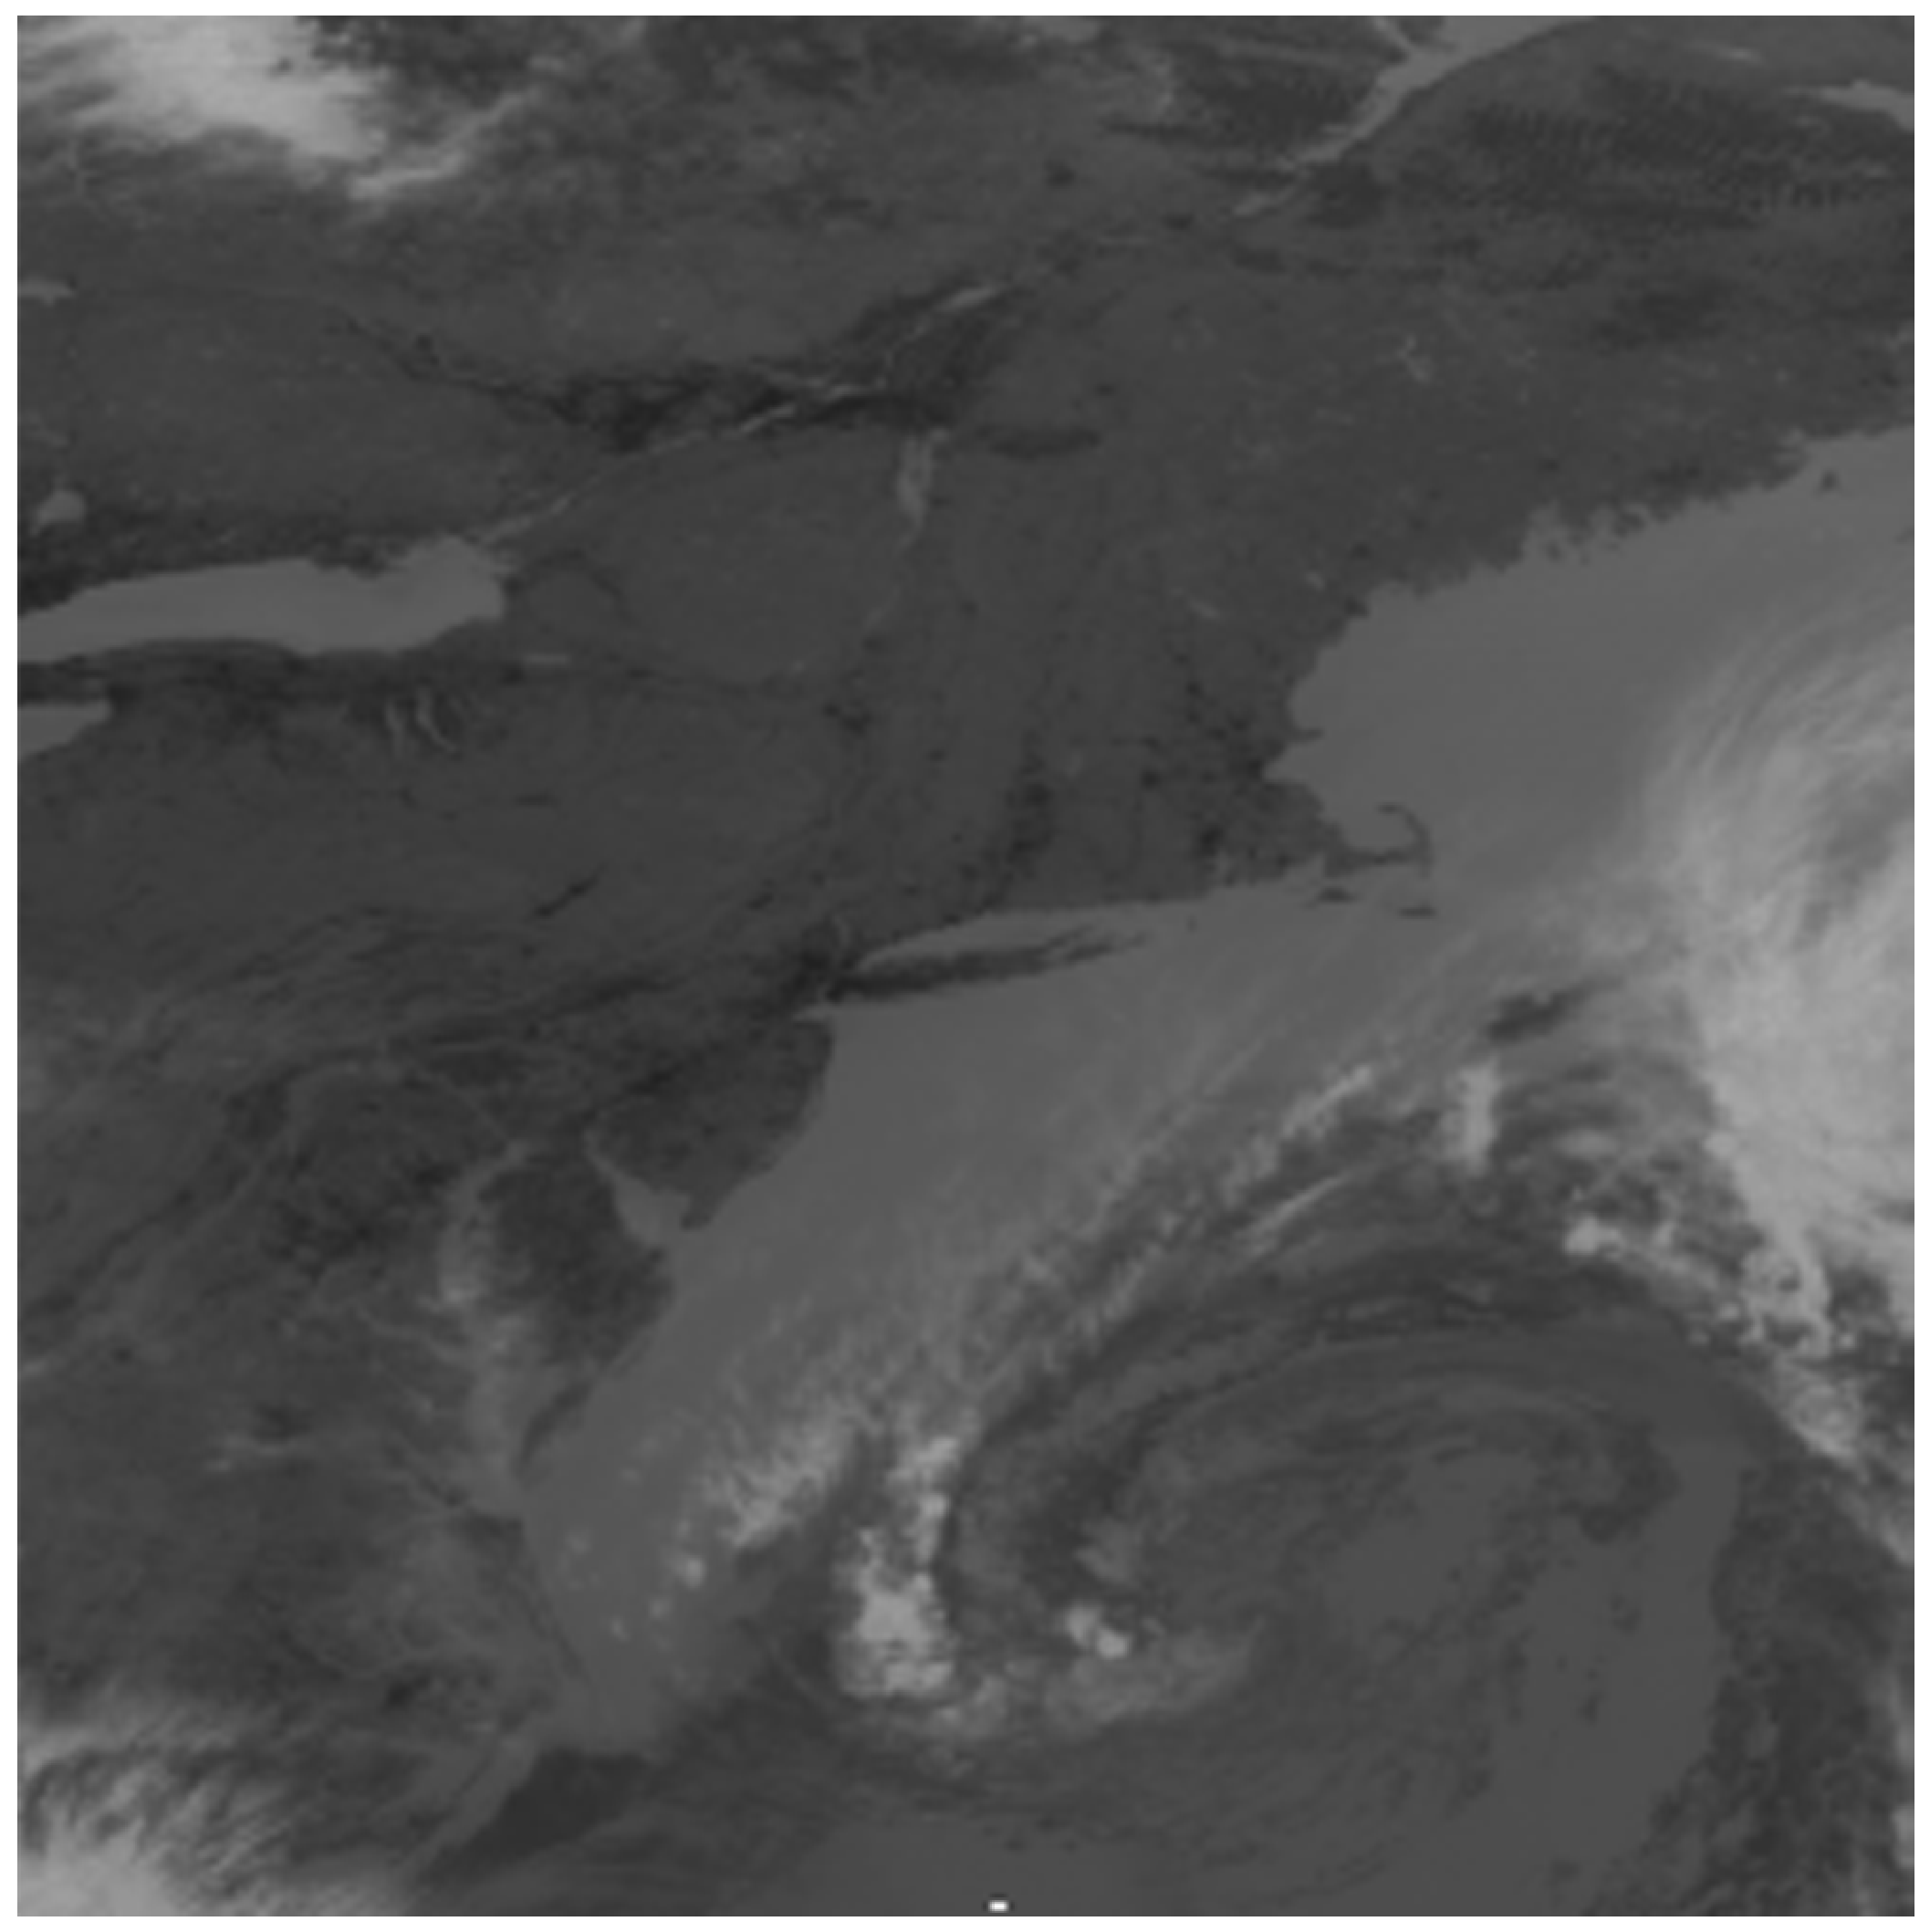
\includegraphics[width=2.5 in]{chl2}
% \label{fig:multichl}
% \end{figure}

\begin{figure}[tb]
\centering
\subfigure[VIS]{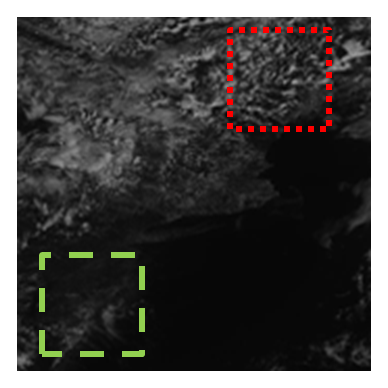
\includegraphics[width=1.06 in]{pics/vis2}
\label{fig:vis}}
\subfigure[Chl2]{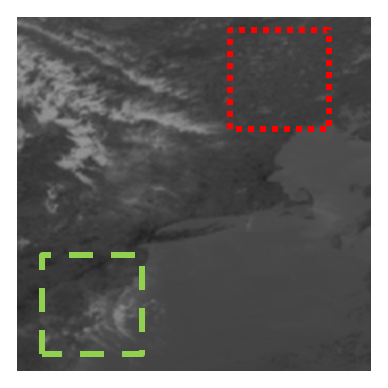
\includegraphics[width=1.06 in]{pics/chl22}
\label{fig:chl2}}
\subfigure[Chl3]{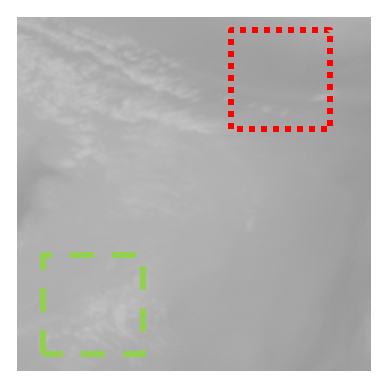
\includegraphics[width=1.06 in]{pics/chl32}
\label{fig:chl3}}
\subfigure[Chl4]{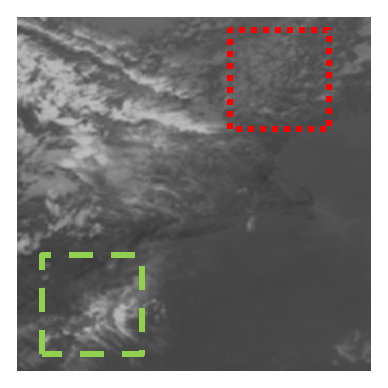
\includegraphics[width=1.06 in]{pics/chl42}
\label{fig:chl4}}
\subfigure[Chl6]{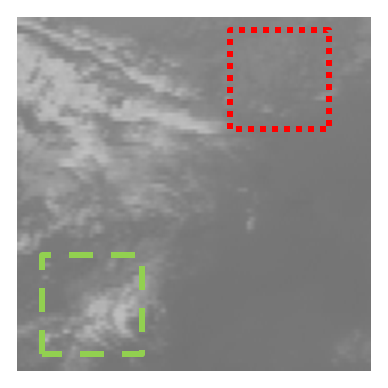
\includegraphics[width=1.06 in]{pics/chl62}
\label{fig:chl6}}

\caption{Multi-channel view: Visible channel fails to capture clouds in
the left-bottom box but other channels do not show clouds on right-top box}

\label{fig:multichl}
\end{figure}


\begin{enumerate}%[(1)]
\item \textbf{Evaluation of motion estimation methods for satellite} 
Most of previous works used the block-wise cross correlation \cite{cote1995neural,leese1970determination}. But in the case of satellite images,
block-wise motion is unable to track small changes of both cloud shape and motion
field. Therefore we propose to use the Optical Flow (OF) 
motion estimation algorithm which is based on the gradient of grey-scale change.
Compared with traditional algorithms such as HBM, it is more sensitive to small 
area change and robust even with shape distortion.

% Limitations of these approaches
% are try to estimate block-wise movements and continuous and/or regular motion vector change trends estimation
% but in case of satellite, 
% tend to generate higher motion estimation error rate because of  but in case of 
% satellite, such block-wise movements are too big and motion vector change trends are 
% not easy to be captured with the HBM. Therefore we propose to use  Optical Flow (OF) 
% motion estimation algorithm which is based on gradient of grey-scale change. 
% Compared with traditional algorithms such as HBM, it is more sensitive to small 
% area change and robust in shape distortion.

\item \textbf{Robust regression analysis for irradiance prediction} 
Most previous works used a variant of the linear regression
model~\cite{perez2002new}.
However, this approach is quite sensitive to noise or outlier. We propose Support 
Vector Regression (SVR) which has several advantages over the ordinary linear regression models. 
First, SVR ignores outlier points, thereby reducing influence of noise from
cloud motion tracking. Second, it can easily model linear and non-linear
relations by choosing different kernels, and have better modeling capabilities with a limited number
of features. We also provide a simple approach to properly normalize solar
irradiance level to remove diurnal  and seasonal affects, so that the subsequent
regression analysis could be simpler.  

\item \textbf{Combining multiple evidences}  
To overcome the limitations of the visible channel, we incorporate other four
available channels from satellite imager system to sense the radiant in the
different spectrum range (Figure \ref{fig:multichl}). Second, we added the
radiation level of the previous timestamp as an additional feature to SVR 
model have better context information.

\item \textbf{Systematic evaluation of whole pipeline} 
We did systematic cross validations on 6 months data, and evaluated 1) the
effects of different cloud motion estimation algorithms, 2) the different irradiation modeling performance from the ground truth cloud 
image to irradiation level, 3) the effects of the integrated system from the motion 
estimation to irradiation prediction of up to five hours,  and 
4) the effects of diverse evidences related to irradiation prediction. 

% We did systematic cross validations and showed an up to 50 \% improvement with
% the prediction accuracy with respect to the baseline and other models used in the comparative experiments.


\end{enumerate}

% the following will be integrated to contribution later to reduce space
In this paper, previous works and potential approaches are discussed in
Section \ref{sec:bg}. In Section \ref{sec:preprocessing}, the preprocessing steps and
SVR method are presented in details.  Section \ref{sec:motionestimation} discusses and compares various motion estimation techniques.  Section \ref{sec:Models} enumerates seven estimation models for the satellite based prediction:  linear and non-linear, regular and SVR and their variations.  Section \ref{sec:result} presents the performance details of the proposed satellite models.
% in term of estimation and forecasting.  
In Section \ref{sec:conclusion}, we conclude
that the new forecast system has significant improvement for the 
medium-term radiation forecast.


\section{Background}
\label{sec:bg}

In early years, Satellite models were originally designed to correlate cloud
coverage with Global Horizontal Irradiance (GHI)~\cite{stuhlmann1990improvement,schmetz1989towards}.
Later works continued this idea, and studied the linear relationship between Direct
Normal Irradiance (DNI) and satellite visible channel~\cite{ineichen1999derivation,hammer2003solar}. 
These models use the term ``Cloud Index" (CI) to represent the optical density derived from satellite data.  Here optical density measures the solar absorption by cloud, and is determined by the observed cloud fraction or coverage.  By using multiple empirical clear sky models,
the local solar energy distribution is derived from satellite
images~\cite{janjai2005development}.  Some recent work refined this modell, and added more parameters/factors, such as terrain factor~\cite{perez2004producing}.   Some new ideas were proposed based on other fields such as statistical approach~\cite{zarzalejo2009new} and
Artificial Neural Network (ANN) method~\cite{csenkal2009estimation}.   
Some related work, for example, ~\cite{csenkal2010modeling} does not even require meteorological data.
In fact, the biggest concern with the satellite-based cloud coverage lies in images from the untrusted and unstable visible channel. As shown in Figure
\ref{fig:multichl}, visible channel sometimes fails to capture cloud and
cannot differentiate cloud types in greyscales. Another concern about
visible channel is that snow coverage and variational floating of image
with various zenith angles, and confuses with the normal cloud cove,  and cauded some difficulties in cloud tracking.  As a
result, multispectral approach is required for further analysis. The basic idea is
to use empirical thresholds on the  multi-channel images of satellite, and then perform cloud
classification and snow detection. 
\cite{perez2010improving,ricciardelli2008physical}.

% the work relies
% on heuristic thresholds for infrared and visible range are needed for 

%  In most satellite approaches, linear relation is derived from cloud coverage to
%  solar radiation. 
 
%   Another drawback of previous works is that simple linear relation derived 
% from cloud coverage has limitations in describing variation under cloudy condition. 
% Therefore, a customized constant must be used as an estimation compensation 
% to reduce linear biased influence \cite{perez2002new}.
To use the satellite model for forecasting, we need to implement a cloud tracking scheme required for predicting the cloud distribution in advance. One of the tracking ideas
is to estimate the movement of cloud. In previous approaches, cloud motion vectors
are generated from blockwise cross-correlation matching
\cite{leese1970determination,heinemann2006forecasting}. But the most
challenging problem comes from the matching technique that oftern assumes the 
invariant texture and constant movement of cloud. In fact, the existing cloud
condition and motion aglorithm is not stable and  becomes even more complicated with satellite images.
Therefore many recent works tried  the no-motion approach, and integrated other sources of information, e.g.  ground radar measurement.  Here the ground radar based 
prediction model obtained the continuous radiation fluctuation pattern for performance improvement ~\cite{gorsdorf2011cloud}.  But those no-motion methods tend to have low precision outcomes and offter only short forecast time.  Since no real cloud tracking is involved, the
forecasting is essentailly a statistical approach and its prediction range is between several minutes and up to 2 hours \cite{yang2012hourly}. 



% It turns out to be
% highly sensitive to block size and segmentation as it tries to represent area of
% cloud in block unit. 
%  
% To build a forecast system, a cloud motion tracking system is needed for Cloud
% motion estimation studies are mostly about cloud prediction.
% To describe cloud distribution in advance, cloud motion vector
% extraction is usually used for estimating cloud movement. As an important input
% parameter to feed satellite models, cloud motion vectors are
% commonly generated from blockwise cross-correlation
% matching~\cite{leese1970determination,heinemann2006forecasting}.  % cite our paper
% It turns out to be highly sensitive to block size and segmentation as it tries
% to represent area of cloud in block unit. 
% In fact, this methodology is based on a basic assumption that cloud motion is stable and identical with no deformation. 
% But in reality, cloud on satellite image is more complicated as with rotation and shape
% changing. Therefore merging and splitting of cloud will be ignored due to fixed
% block size. Another extreme case is that when multilayer clouds appear, block
% matching will fail as its correlation only covers the texture information in a
% block. Therefore a lot of recent works tried evade the unsolved issue of cloud
% motion by integration of other source of information, e.g. radar ground measurement.
% One way to to predict cloud ahead is using ground radar to get continuous
% radiation fluctuation trend~\cite{gorsdorf2011cloud}. Yang et. al~\cite{yang2012hourly}
% explored the time series feature of cloud statistically to do
% prediction. The drawbacks of no-motion based methodology is that
% cloud tracking is of low precision and forecast time can only be either minutes 
% or up to 2 hours as they claimed.
% 
% Though satellite approach is also in mesoscale, local information can be
% assimilated through adding ground-based pyranometer and multispectral
% views. Another drawback of current models is that the precision in
% both temporal and spacial accuracy decrease rapidly with the longer forecast
% period. 
% 
% The irradiance modeling from estimated satellite cloud is more accurate
% than methods that interpolating data measured by a modern radiometric network, \cite{zelenka1999effective},
% and thus many works regarding mesoscale range (30 minutes to five hours) have been developed using satellite data. 
% % 

% In our approach, we target to use the ground-based pyranometer and
% satellite images to get estimated radiation in future. The local instrument such as pyranometer
% can provide Direct Normal Irradiance (DNI) per second while satellite images
% have 30 minutes response time before next scanning. Due to this, radiation prediction
% may start from 30 minutes to five hours. Compared to pyranometer, 
% the satellite images have much lower lower spatial resolution (1 km x 1 km in visible
% channel, 4km x 4km in infrared channels), especially in multispectral
% and motion vector related applications. %To meet the requirement of local station forecast, pyranometer data is assimilated into satellite model as another feature. 


\section{Data Preprocessing} % 1) need better name 2) re-consider
% better place to put this section
\label{sec:preprocessing}

Due to the limitation of remote sensing techniques,
we have to use all available evidences to reduce abnormalities brought from
satellite data. Therefore we expand preprocessing work to multi-channel instead
of just visible channel of satellite. From the dataset collected by GOES project
\cite{GOES:2013:Online}, we found several frequent error patterns: 1) black rasters of multispectral images due to failure
of sensing or raw data processing, 2) luminance variation, especially on visible
channel, and 3) missing channel data. We used empirical filters such as mean
filter to fill out black raster lines and bad-frame filter to remove low quality
or missed frames. We normalized the brightness according to solar zenith angle. 
The overview of data preprocessing is shown in Figure \ref{fig:satpre}. 
% SJ: I'm not so much clear on this figure

Another key step in preprocessing pipeline in the Figure \ref{fig:radpre} is
handling radiation data measured by pyranometer. There are two concerns: 1) radiation level
normalization from bell shape curve to uniform level to avoid daily and seasonal
effects and 2) different temporal resolution resolving between satellite (30 minutes) and pyranometer 
(one second). In previous works, clear sky irradiance is calculated by clear sky
models which are based on based on atmospheric parameters such as O2, CO2,
Ozone, water vapour and aerosol optical thickness
\cite{perez2002new}. However, such models are sensitive to
the location and ask additional input variables. To address this concern, 
we propose to use polynomial regression to generate the monthly clear sky
radiation curve shown in Figure \ref{fig:csfig}. Then we calculate
normalized radiation at $t$ using the average of $[t-N,t+N]$ minutes
radiation divided by the average of clear sky values. 
Normalization using average over $2N$ minutes minimizes
the influence of temporal resolution mismatch and smoothes out short-term local
irradiance fluctuation. 

% normalized radiation to avoid the temporal resolution mismatch
% between satellite and ground base station. The routine satellite scan is 30 minutes while the pyranometer sampleing rate is one second unit. As a result, the timestamp of satellite is not exactly matching to ground based irradiance sensor output.  By taking the irradiance average around $N$ minutes, it smoothes out the irradiance local fluctuation.
% As measured irradiance is fluctuating with cloud distribution,
% cloud effect on total irradiance can be measured by normalization with
% clear sky irradiance. 
% 
% requires clear day irradiance but it may be difficult to
% get a perfect clear sky data and most clear sky models
% \cite{janjai2005development,perez2002new} are based on atmospheric
% parameters such as O2, CO2, Ozon, water vapour and aerosol optical thickness.
% However, such models are sensitive to the location and ask such addtional input
% parameters. To overcome these problems, we propose to use poynomial
% regression for the monthly clear sky radiation curve shown
% in Figure~\ref{fig:csfig}.
%	zhenzhou: I used more than 2-order polynomial regression in application.

\begin{figure}[tb]
\centering
\subfigure[Satellite Preprocessing]{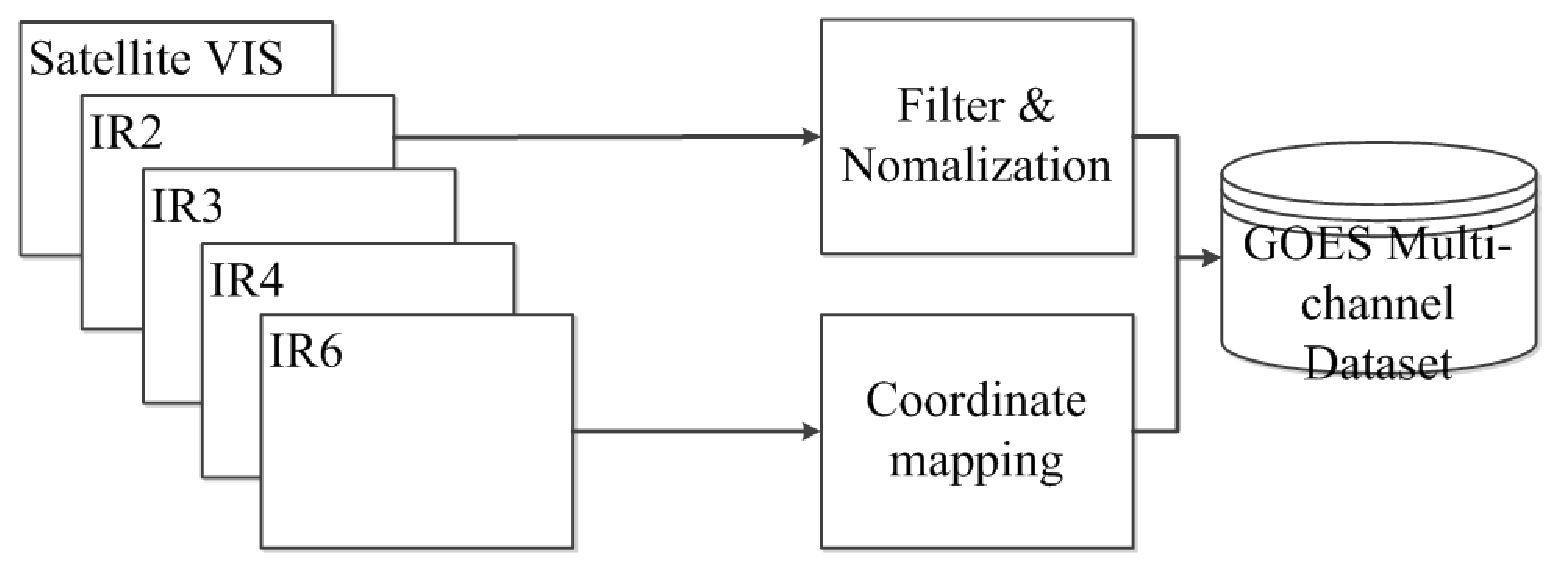
\includegraphics[width=3 in]{pics/satpre}
\label{fig:satpre}}
\subfigure[Irradiance Preprocessing]{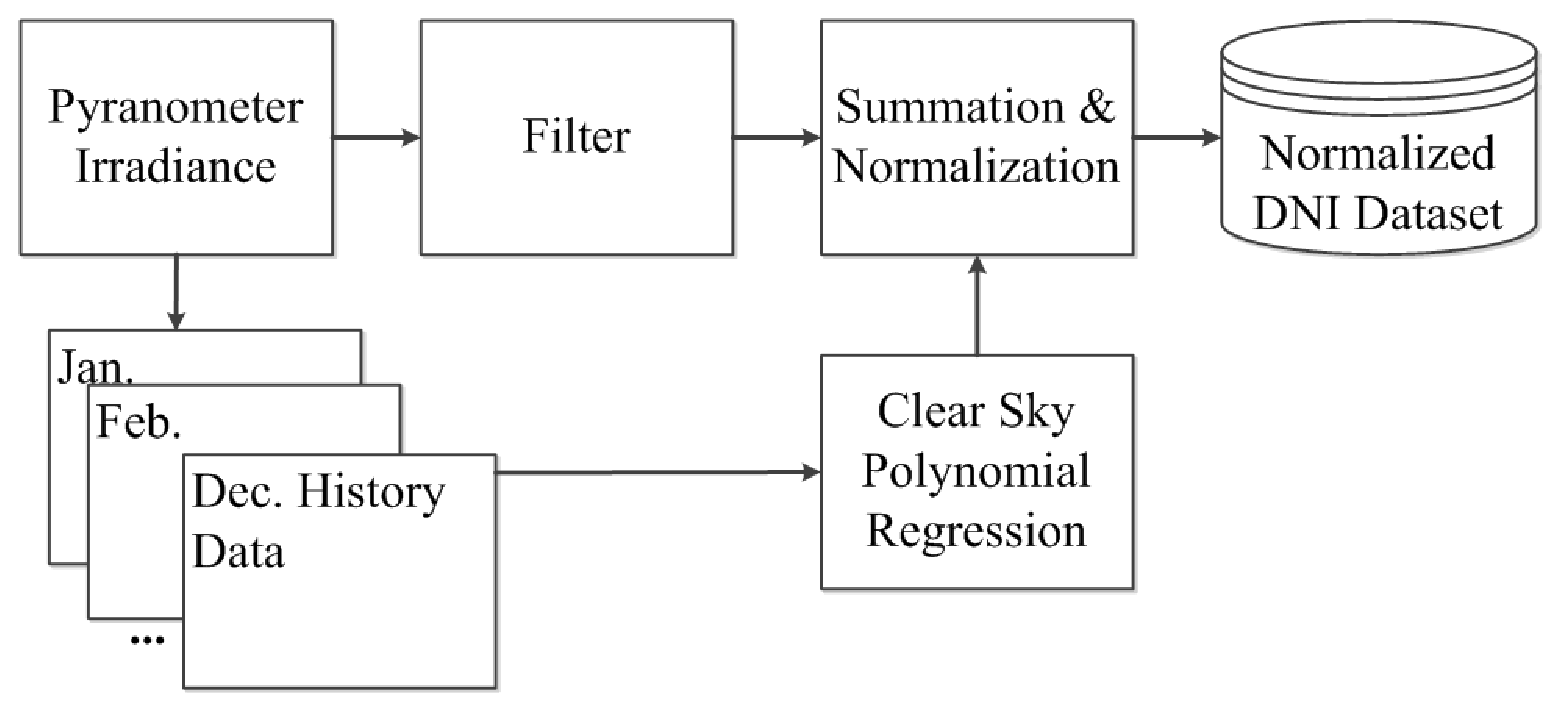
\includegraphics[width=3 in]{pics/radpre}
\label{fig:radpre}}
\caption{Data Preprocessing Framework}
\end{figure}

%
\begin{figure}[tb]
\centering
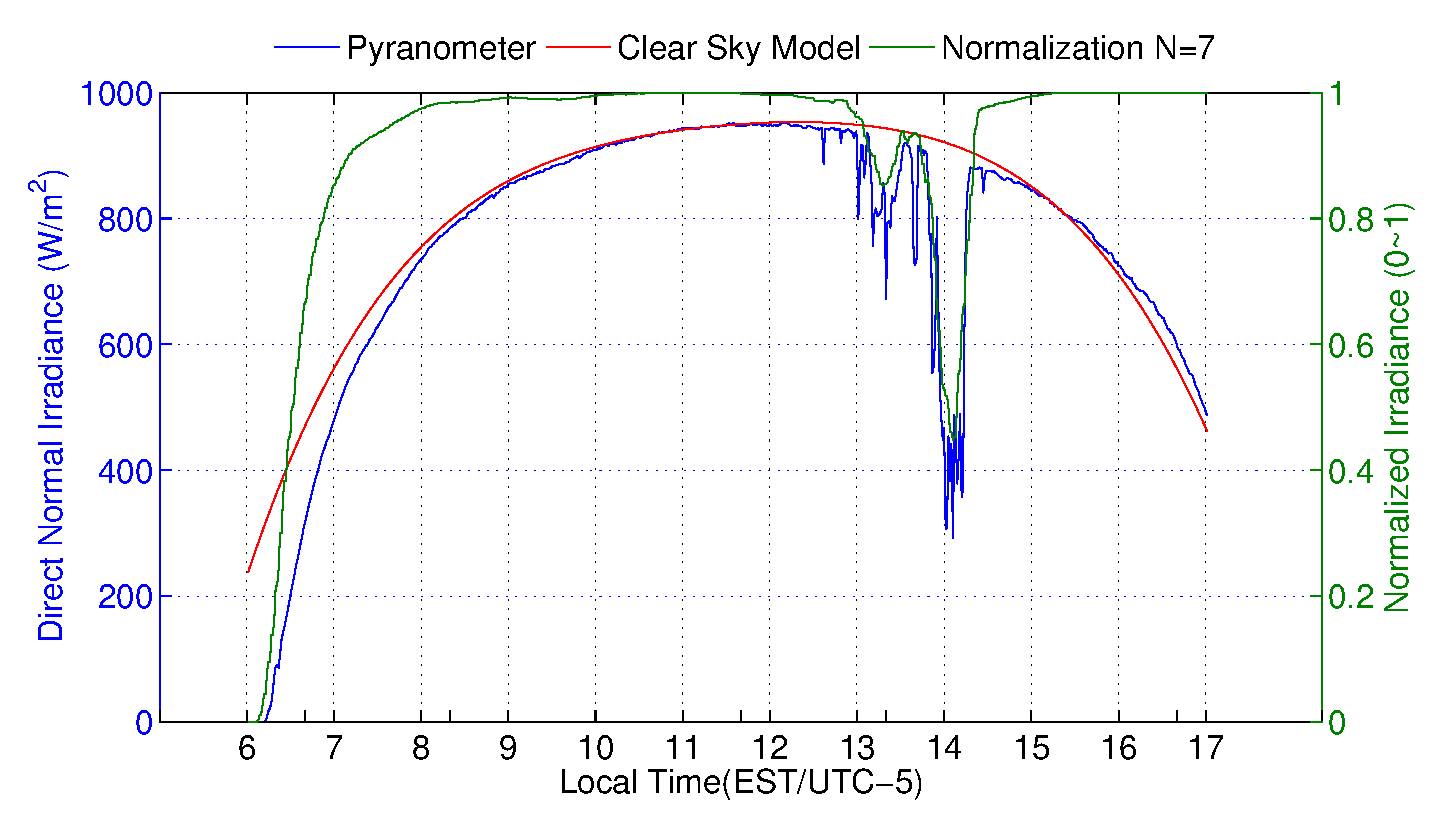
\includegraphics[width=3.2 in]{pics/csfit}
\caption{Irradiance normalization and clear sky profile on March 1st, 2012}
\label{fig:csfig}
\end{figure}
%
% and it also helps to spatial resolution difference. <--- need additional explanations

% \begin{figure}[tb]
% \centering
% 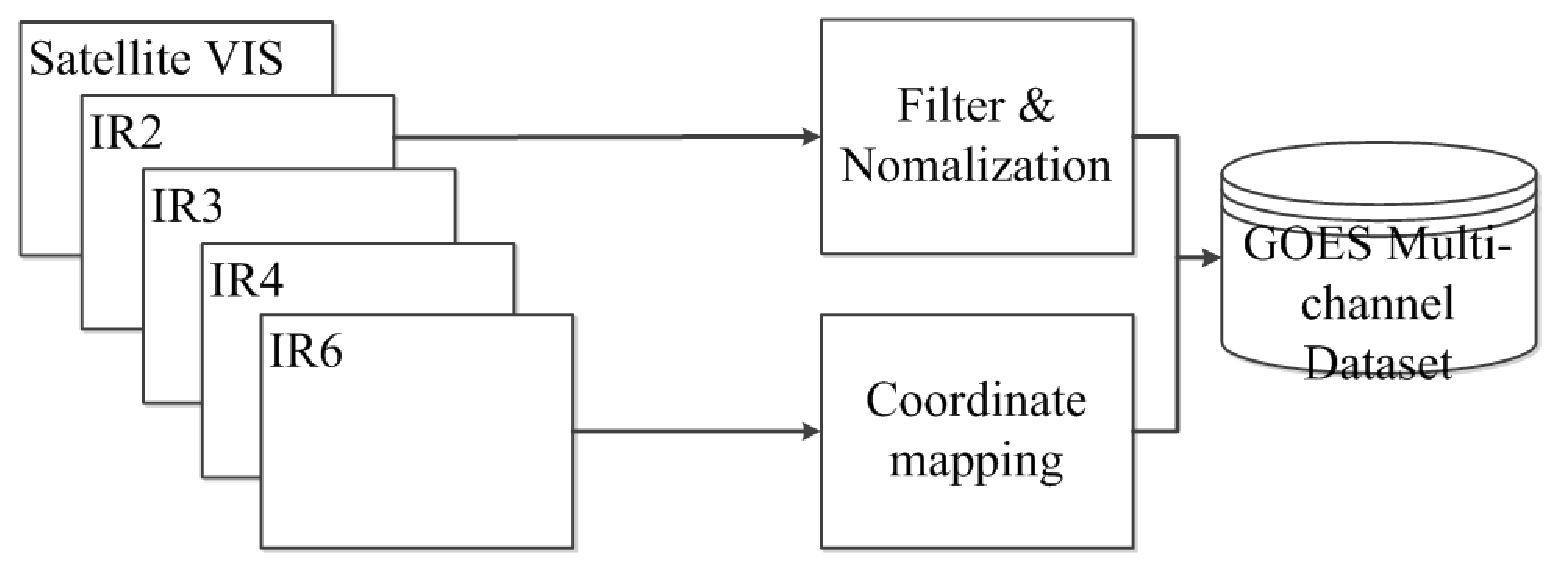
\includegraphics[width=3 in]{pics/satpre}
% \label{fig:satpre}
% \caption{Data Preprocessing Framework}
% \end{figure}





\section{Motion Estimation}
\label{sec:motionestimation}
%%
% SJ: Zhenzhou please consider to merge the next paragraph with Background's the first paragraph because they are repeating...
%%
The sequence of satellite images provide motion information of cloud field and
allow us to predict distribution in near future. For this, the motion estimation
algorithms play a crucial role for irradiance forecasting. In image processing
and multimedia field, a well studied approach is Hierarchical Block
Matching(HBM) which is on the basis of similarity check among blocks. It is
widely used in video coding and compressing as its properties of fast speed and
high compressing ratio. As to accuracy, the performance lies on region size and
feature matching which assumes consistence of image segmentation. For
satellite image case, cloud variation should be considered in
smaller scale instead of blocks. Therefore we propose to use pixel-wise
approach.


% In order to
% address uncertainty of cloud variation, we propose another approach which focus
% on pixels rather than blocks.

% In other words, block-matching performance suffers from uncertainty of cloud variation and highly relies on selected block size.
% image. Therefore block-wise approach is not stable and much worse in terms
% of small scale motion tracking. To get rid of these issues, we
% propose to use Optical Flow algorithm.

Optical flow (OF) motion estimation is a branch of methodologies that utilize
the gradient of image. Under the assumption of constant illuminance, displacement of
pixels will be estimated following gradient change. The implementation of OF
idea has a lot of variations as gradient of image is defined differently. In our
approach, we choose Lucas-Kanade Optical Flow(LKOF)~\cite{lucas1981iterative} as
the tracking method. For robustness, we implement a pipeline which
builds the pyramid of image. The framework of pipeline is presented in Figure
\ref{fig:OFME}.

In general, visible channel image is firstly scaled to different resolution
levels to build pyramid of image (i.e. 1000x1000 and 500x500). For each level,
motion vectors are computed in turn, following gradient starting from
pre-knowledge of motion. The start motion vectors are the output
of motion from last level in pyramid. When the last level completes
motion vector extraction, we utilize this as pre-knowledge of motion on
original size. Then the final motion vector is found by seeking for local minima
following the gradient recursively. As image prediction based on
the pixel-wise motion vector will generate ``black hole'' due to moving
of pixels. we apply mean filter on the OF pipeline output to be our
$OF_{mean}$ method so as to reduce information loss.
 



% levels will take their Different
% from top level, the motion vectors starting from level 2 take previous output as initial motion vectors for gradient calculation. Then the output of the last layer which is of
% highest resolution, will be used as starting motions for recursive motion extraction following illuminance gradient changes to find optimal motion vectors. 
%   In addition, Since the cloud texture moves following the motion vector will generate 
% ``black hole'' in original position in predicted image. To reduce the influence
% of information loss, we apply mean filter on the OF pipeline output to be our
% $OF_{mean}$ method.



% In addition, the image prediction highly relies on the prediction accuracy of
% true motion and information loss after movement. In fact a deviation from true motion is
% exponentially accumulated with time in prediction procedure.
% Since the cloud texture moves following the motion vector direction, original spot will
% be left as black-hole resulting that no information is provided in prediction.
% Especially, a larger movement leads to more information loss.
% The motion estimation output of OF pipeline, therefore, may be insufficient in terms
% of information loss. As a result, a mean filter is used to fill black holes in image 
% prediction to increase robustness. 

% for initial motion extraction for each pixel. As higher layer has lower
% resolution, same view range in lower layers appear to be larger in pixel range due to scaling. Therefore each layer takes pixel-wise motion of upper layer as initial block-wise movement and do Optical Flow motion detection following the gradient.
% At last, image pyramid output is .
%%
% SJ: Zhenzhou, please explain recursion in detail here, so that others can follow what you're saying.
%%

% is used as initial movement of block in current layer Since each individual pixel in higher layer is in fact a block in the following layers, pixel-wise motion generated in previous layer stands for the
% block movement in later layer. With the initial movement information of blocks,
% each layer carries out OF motion estimation in pixel units for later usage. Then
% with pyramid structure of motion extraction, output motion is in pixel-wise and
% a combined result of its neighbors. At last, pyramid's output is used as
% starting motion for recursive motion estimation following illuminance gradient
% change to find final motion vector. The idea of this pipeline is presented in
% Figure \ref{fig:OFME}.



Intuitively, OF pipeline and HBM outputs can be compared using predicted
images.
As is shown in Figure \ref{fig:mecmp}, in one hour image sequences, OF method
is much more robust in terms of tiny texture changes and clouds diminishing. 
HBM is suffering over-estimated problems as in dash-block case and more information
loss such in dot-block case. In terms of whole image deviation from ground
truth, the HBM Mean Absolute Error(MAE) in greyscale is much more than Optical
Flow approach, especially when prediction time is over 3 hours (Figure
\ref{fig:dfdall}).
In addition to pixel-based or image quality based evaluation, we evaluate irradiance prediction 
performance using two approaches compared to ground measured solar radiation. 
%In Section \ref{subsec:MEEval}, we propose to use SVR satellite model as another criteria for performance test in real forecasting.

% errors in In one hour image sequence, OF is more
% suitable to evaluated by comparing predicting the future image sequence with ground-truth satellite visible channel data(Figure \ref{fig:mecmp}).
% In one hour prediction result, OF is more suitable for texture tiny changes and   
% As a result, the HBM is suffering the various change of cloud area especially in
% long time prediction. After 4 hours, image tend to have more abnormal
% overestimation such as green-dot block area and failures of actual cloud
% tracking as the case in red-dash block. Besides regional defect brought from
% block movement, in terms of the whole image, the Mean Absolute Error(MAE)
% from reference image sequence is much more than Optical Flow approach(Figure \ref{fig:dfdall}).
% But the comparisons based on predicted images are just pixel-based or image
% quality based evaluation. To measure goodness of motion estimation algorithm for
% satellite forecast application, irradiance-level verification is needed for localized
% evaluation on the basis of ground measured solar radiation. In section
% \ref{subsec:MEEval}, we propose to use SVR satellite model as another criteria
% for performance test in real forecasting.


\begin{figure}[tb]
\centering
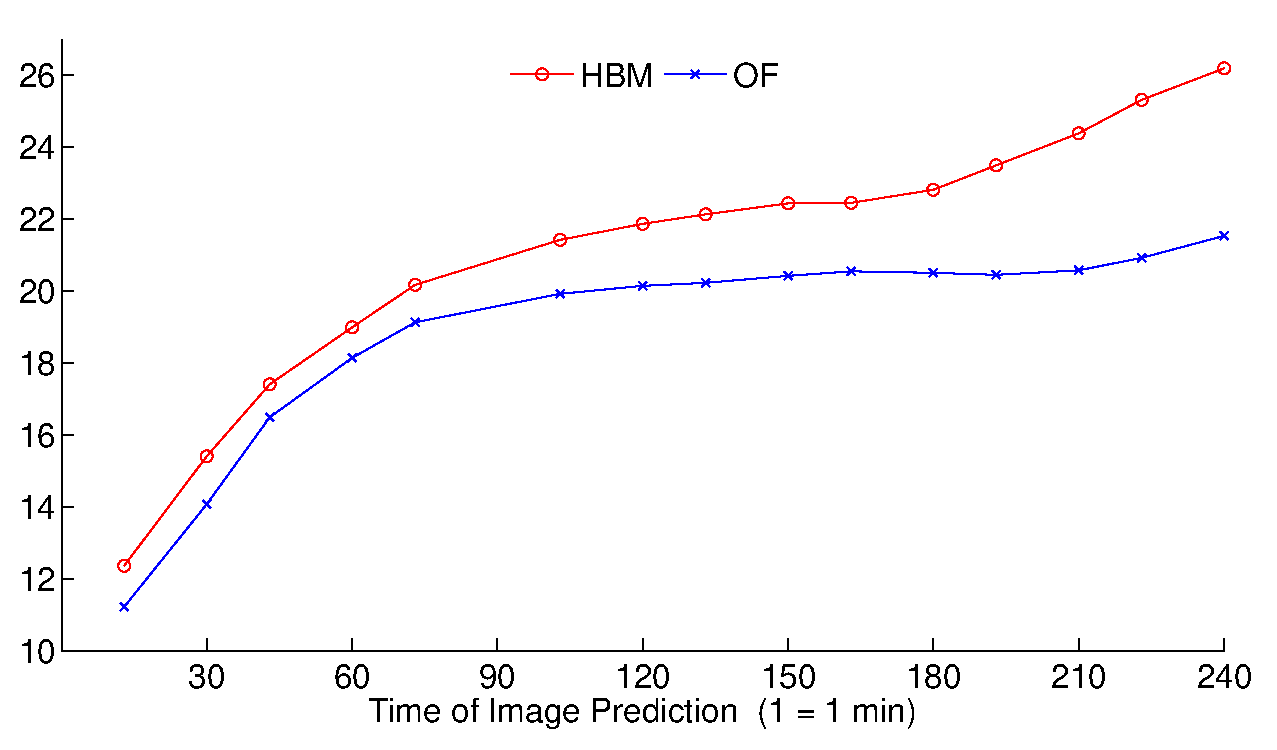
\includegraphics[width=3.2 in]{pics/DFD_all}
\caption{Motion estimation result comparison against ground truth images (MAE) : OF is much better than
HBM with longer prediction time}
\label{fig:dfdall}
\end{figure}



% as OF tracking is applied for detecting motion vectors on smallest image first.
% This motion vector will be initial motion
% vector to the next bigger image layer. The final layer is normally with no scaling 
% and OF is recursively done with the direction of gradient change. % need better explanations
% Then the final motion vector
% map is generated for each pixel. In reality, window size and number of layers
% need be to tuned. The overview of pipeline is presented in Figure \ref{fig:OFME}.

\begin{figure}[tb]
\centering
\includegraphics[width=3.4 in]{pics/ofpipeline}
\caption{Optical flow motion estimation pipeline}
\label{fig:OFME}
\end{figure}


% \begin{figure}[tb]
% \centering
% \subfigure[ground-truth image
% sequence]{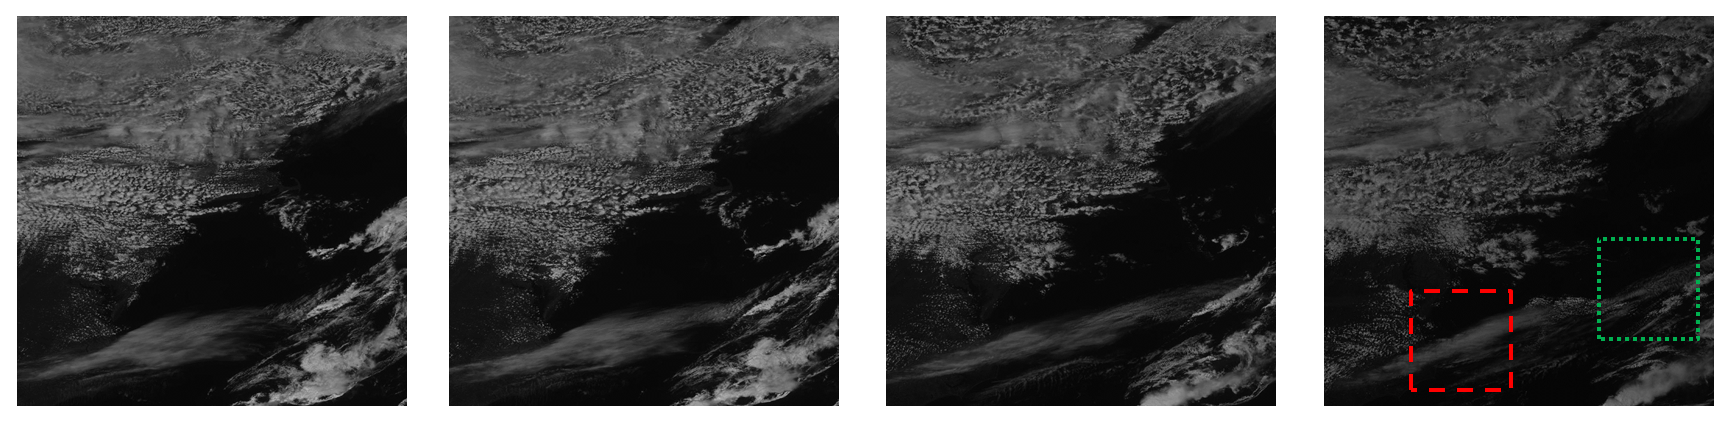
\includegraphics[width=3in]{pics/ME_ori}
% \label{fig:meori}}
% \subfigure[HBM]{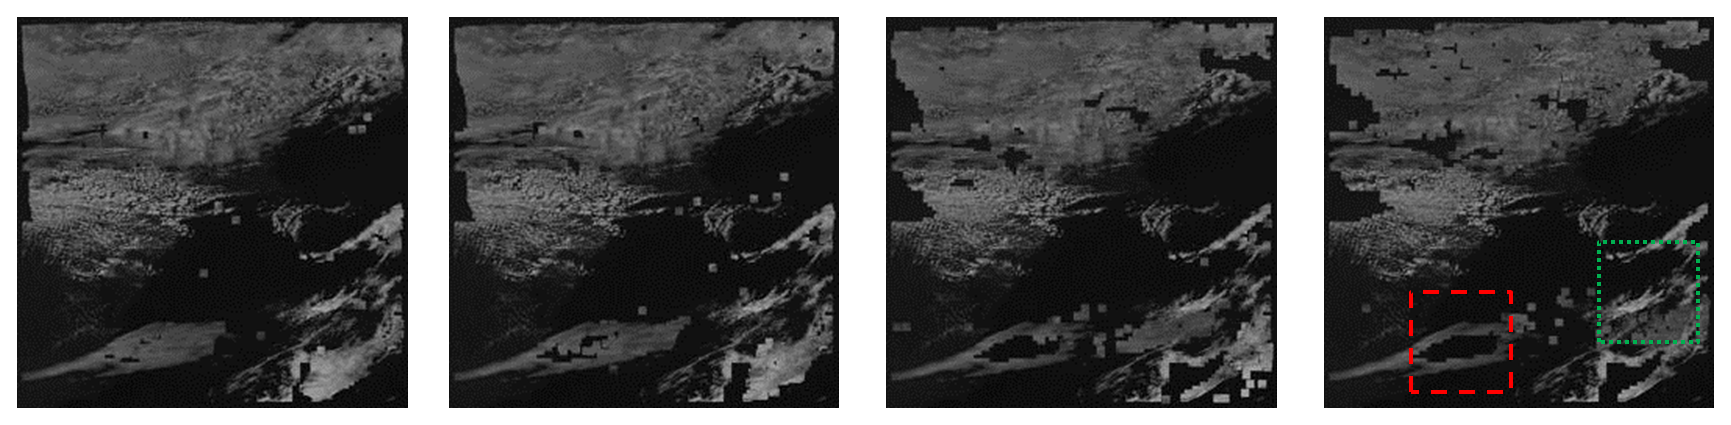
\includegraphics[width=3in]{pics/ME_2f}
% \label{fig:me2f}}
% \subfigure[Optical Flow Motion
% Estimation with mean filter]{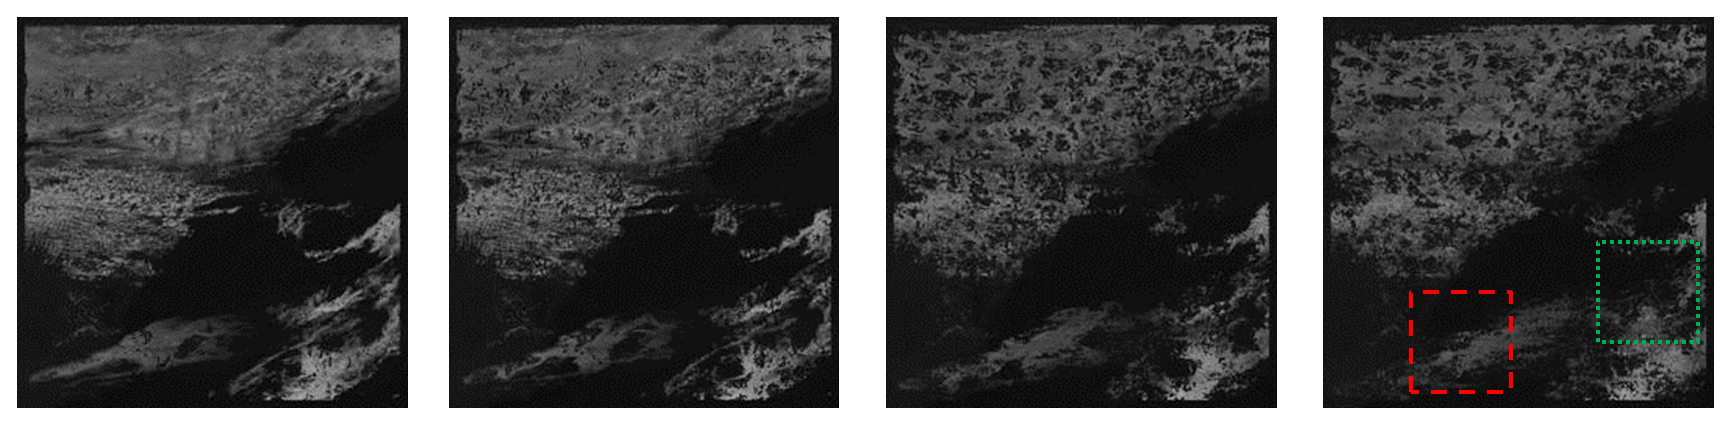
\includegraphics[width=3in]{pics/ME_of}
% \label{fig:meof}}
% \caption{Image Prediction of 0.5, 1, 2.5, 4 hours}
% \label{fig:mecmp}
% \end{figure}
\begin{figure}[tb]
\centering
\subfigure[current frame]{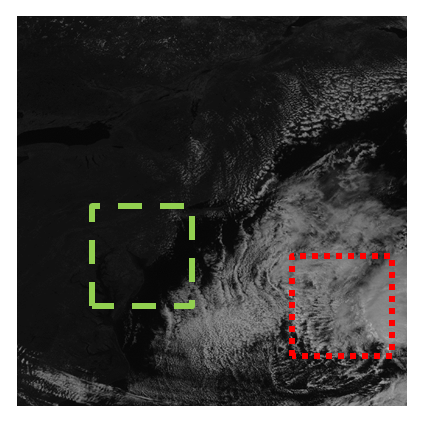
\includegraphics[width=1.6in]{pics/ME_orino}
\label{fig:meorino}}
\subfigure[1 hour later frame]{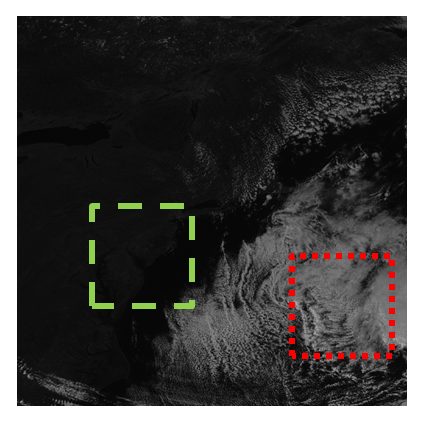
\includegraphics[width=1.6in]{pics/ME_ori1hr}
\label{fig:meori}}
\subfigure[HBM]{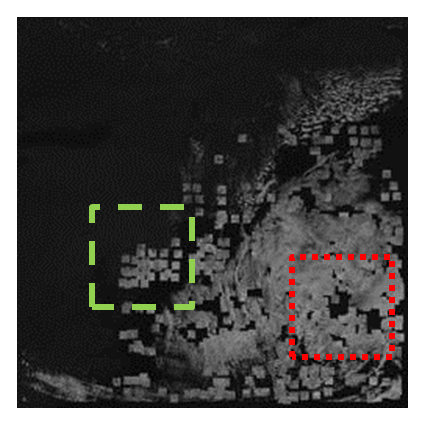
\includegraphics[width=1.6in]{pics/ME_2f1hr}
\label{fig:me2f}}
\subfigure[OF]{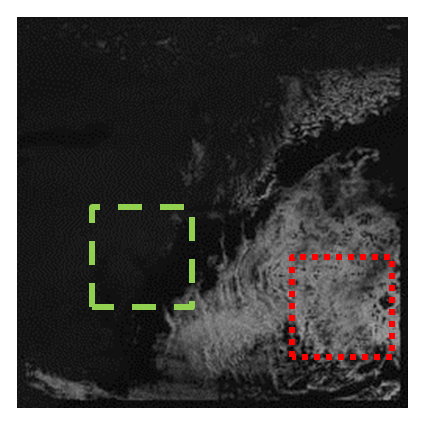
\includegraphics[width=1.6in]{pics/ME_of1hr}
\label{fig:meof}}
\caption{Image Esimation of 1 hour later from (a). With reference to
ground-truth frame (b), (d) captures more texture changes in red
window and is more robust to noise in green window than (c).}
\label{fig:mecmp}
\end{figure}



\section{Radiation Prediction Models}
\label{sec:Models}

Given the satellite images, we may model irradiance from the cloud properties at a point of our interest on the ground.
Our goal is to find a method that 1) utilizes multiple evidences such as multi-channel features and previous timestamp irradiance
and 2) is robust to the noise coming up from preprocessing and motion estimation.
In this Section, we will investigate the simplest Cloud Index (CI), Linear
Regression (LR, ALR) and  Support Vector Regression (SVR).

\textbf{Cloud Index (CI)} 
Cloud Index (CI)~\cite{perez2002new} is a widely used estimation model on the
basis of linear relation between single channel (visible channel) with radiation. CI for a sample time point $i$ is defined as:
%
\begin{equation}
CI_i=\frac{x_i-bound_{min} }{bound_{max}-bound_{min}}
\end{equation}
%
where $x_i\in[0,255]$ is a visible channel value and $bound_{min}$ and
$bound_{max}$ are minimum and maximum observed $x$ value. In other words, $CI_i$ is a normalized
cloud level between zero and one. Given $CI_i$, the irradiance is calculated:
%estimation
\begin{equation}
y_i=w \cdot (1 - CI_i)+b
\end{equation}
where $w$ is the maximum radiation level which is one in our case due to irradiance normalization 
and $b$ is called the compensation value which is learned by the training data.
%
Cloud Index model is just the observed visual channel output to be rescaled to the radiation level
with the compensation value to correct bias.
There are couple of problems of this simple method. First of all, CI model will suffer from illuminance changes with solar zenith angle.
Due to this problem, we preprocessed the satellite image to be normalized with zenith angle for all of our model input.
Second, we can only fit the bias term, so that it can not be fitted well with the data.
Third, CI model used only single channel, which means we can not combine the other available evidences.

\textbf{Linear Regression (LR, ALR)}
The straight forward extension of CI model is Linear Regression (LR) and
Aggregate Linear Regression (ALR) using multiple channels as extra evidence.
\begin{equation}
y_i = \mathbf{w \cdot x_i} + b 
\end{equation}
where $\mathbf{w} \in R^d$ is a row weight vector and $\mathbf{x_i} \in R^d$ is a column vector for the input, 
and $b$ is the intercept. The advantages over CI model are that LR models may
include multiple evidence as linear relationship and both $\mathbf{w}$ and $b$ are learned from the training data to be better fitted.
But LR is suspectible to the noise because of the least square objective function
to find optimal $\mathbf{w}$.
\begin{equation}
 \underset{\mathbf{w},b}{\text{min}} \sum_i{(\mathbf{w}\cdot \mathbf{x_i} + b - y_i)^2 } 
\end{equation}
If there are outlier points, then $\mathbf{w}$ will be overfitted.

\textbf{Support Vector Regression (SVR)}
To avoid such overfitting from noisy data, we propose to use Support Vector Regression (SVR) as our solution.
\begin{equation}
 \underset{\mathbf{w},b,\xi,\xi^*}{\text{min}} \frac{1}{2}\|\mathbf{w}\|^2  + C {\sum_{i=1}^{n}\left(\xi_i + \xi_i^{*}\right)}
\label{pm:svr}
\end{equation}
subject to 
\begin{equation}
\begin{aligned}
(\mathbf{w \cdot x_i} + b) - y_i &\le \varepsilon + \xi_i, \xi_i \ge 0 , \forall i\\
(\mathbf{w \cdot x_i} + b) - y_i &\ge - \varepsilon - \xi_i^{*}, \xi_i^{*} \ge 0 , \forall i
\end{aligned}
\label{pm:svrc}
\end{equation}
where $\varepsilon$ is the margin for regression, $\xi_i$ and $\xi_i^{*}$ are slack variables, and $C$ is a regularization parameter. 
Then, the predicted irradiance will be 
\begin{equation}
\begin{aligned}
y_i = \mathbf{w \cdot x_i} + b & \text{ if } 0 \le y_i \le 1\\
0 & \text{ if } y_i < 0 \\
1 & \text{ if } y_i > 1 
\end{aligned}
\end{equation}

The basic idea of SVR is the regression error to be within $\varepsilon$. 
If it can not be learned within $\varepsilon$ bound, 
the slack variables allow us to fit the model out of $\varepsilon$ bound 
but the slack variable has to be minimized with $C$ regularization term, Equation \ref{pm:svr}.
Since it bounds errors to be within $\varepsilon$, it is much more robust and 
it is easy to extend non-linear relationship using kernel trick, which projects
data into high dimensional space, so that we could model non-linear relationship
with linear model\cite{smola2004tutorial}. We used RBF (Radial Basis Function) kernel:
\begin{equation}
k(\mathbf{w'},x)=\phi(\mathbf{w'}) \cdot \phi(\mathbf{x}) = e^{-\frac{\parallel \mathbf{w'-x} \parallel^2}{2\sigma^2}}
\label{rbfkernel}
\end{equation}
where $\sigma$ is a tuning parameter for the smoothness of RBF kernel.

%\textbf{Combining Evidences}
For ALR and SVR, we considered not only visible channel but also the remaining
four channels and the previous timestamp irradiance value as the context information.
By combining multiple channels, we can overcome the limitations of visible channel and have better cloud distribution information from the other channels.
We will evaluate the different evident effects in the next Section.

 
\section{Experiment Results} % 1) need better name 2) re-consider better place to put this section
\label{sec:result}

\subsection{Dataset}
\label{subsec:dataset}
We collected satellite dataset from April 1st 2012 to November 1st 2012, 
covering partial spring, full summer, and most autumn. The radiation data is
from pyranometer on-site measurement from Brookhaven National Laboratory.
For both satellite images and pyranometer measurements, the raw input
data has been preprocessed by removing data points which have 1) any bad-frame of multi-channels
2) failure of ground radiation sensor 3) multi-channel timestamp mismatch and 4) low
solar angles. In total, we extract daytime dataset which has 8477 frames for
each channel and radiation timestamp continuously. Each radiation data point is
a result of normalization and average value in range of 15 minutes. The detailed
information of dataset is summarized in Table \ref{tab:dataset}.

\begin{table}[htb]
\caption{Satellite dataset}
\centering
\label{tab:dataset}
    \begin{tabular}{   l  |  l  |  l  | l }
    \hline
   Dimension	&size	&temporal resolution	&spatial resolution  \\ \hline
   Channel 1	&8477   &15min,30min			&1km x 1km    \\ \hline
   Channel 2,3,4,6	&8477   &15min,30min		&4km x 4km    \\ \hline
   radiation	&8477   &15min			&NA    \\ \hline 
   \hline
    \end{tabular}
\end{table}


\subsection{Parameter Tuning and Evaluation Metrics}
\label{subsec:esti_e}

For whole dataset, we used five-fold cross validation to split training and testing 
and used five-fold cross validation again to tune model parameters within
training data. In our experiment, Mean Square Error (MSE) and Mean Absolute
Error (MAE) are used to evaluate the predicted model accuracy.
They are defined as:
% We tuned $C$ from 0.1 to 1000, $\varepsilon$ from 0.001 to 0.1 and $\sigma$ of
% RBF kernel from 0.1 to 1000.
% The final tuning shows best $c = 32$, $\varepsilon = 0.01 $ for Linear kernel
% and $c = 1$, $\varepsilon = 0.005 $, $\sigma = 22.62$ for RBF kernel.
 

%
\begin{equation}
\label{eq:MAE}
MAE=\frac{1}{N} \sum_{i}\left | \hat{y_i} - y_i \right |
\end{equation}
%
\begin{equation}
\label{eq:MSE}
MSE=\frac{1}{N} \sum_{i}{(\hat{y_i} - y_i)^{2}}
\end{equation}
%
where $\hat{y_i}$ is the predicted radiation level, and $y_i \in [0,1]$ is the ground truth radiation level.
Note that the radiation level is normalized by clear sky irradiance value. 
%
\begin{figure}[tb]
\centering
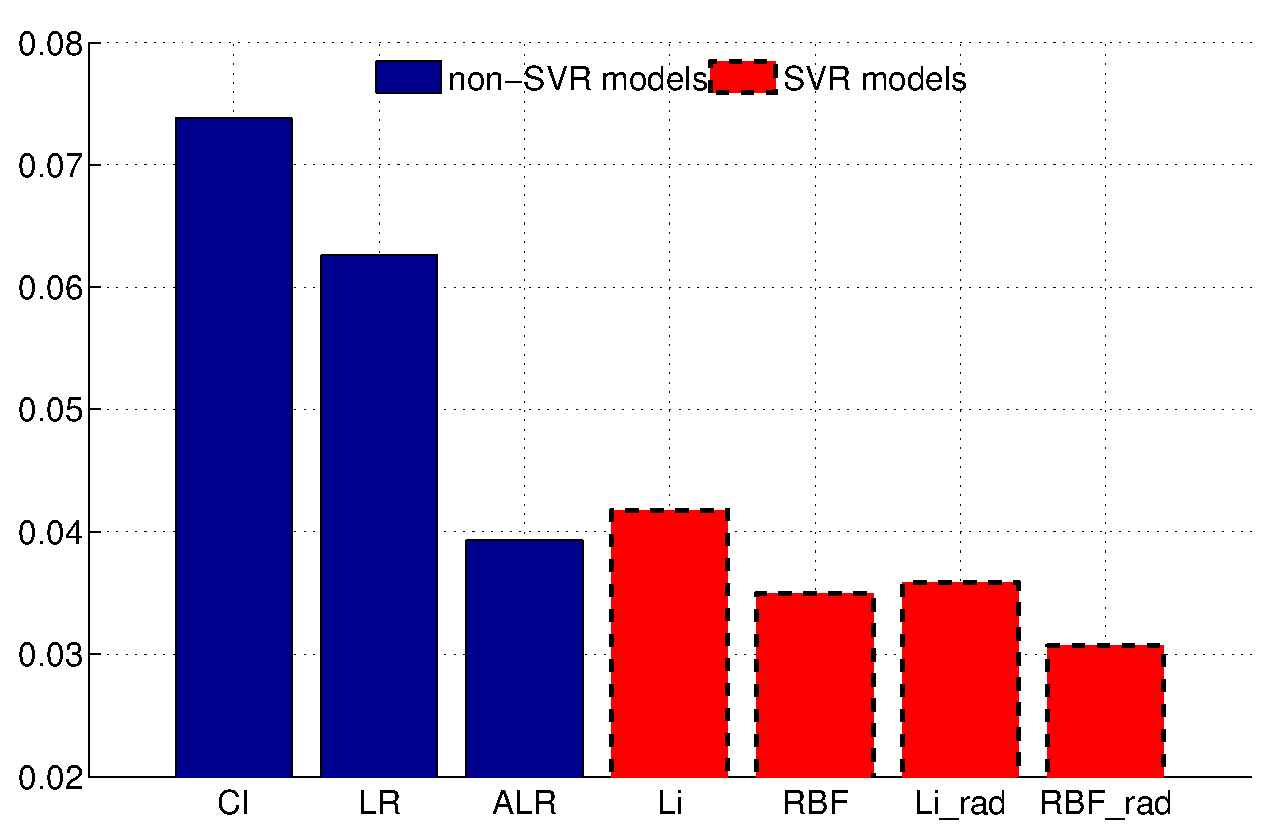
\includegraphics[width=3.2 in]{pics/modelsmse2}
\caption{MSE Plot of 5-fold cross validation. SVR models show less amounts of errors than non-SVR models in general.}
\label{fig:modelsmse}
\end{figure}
%
\begin{figure}[tb]
\centering
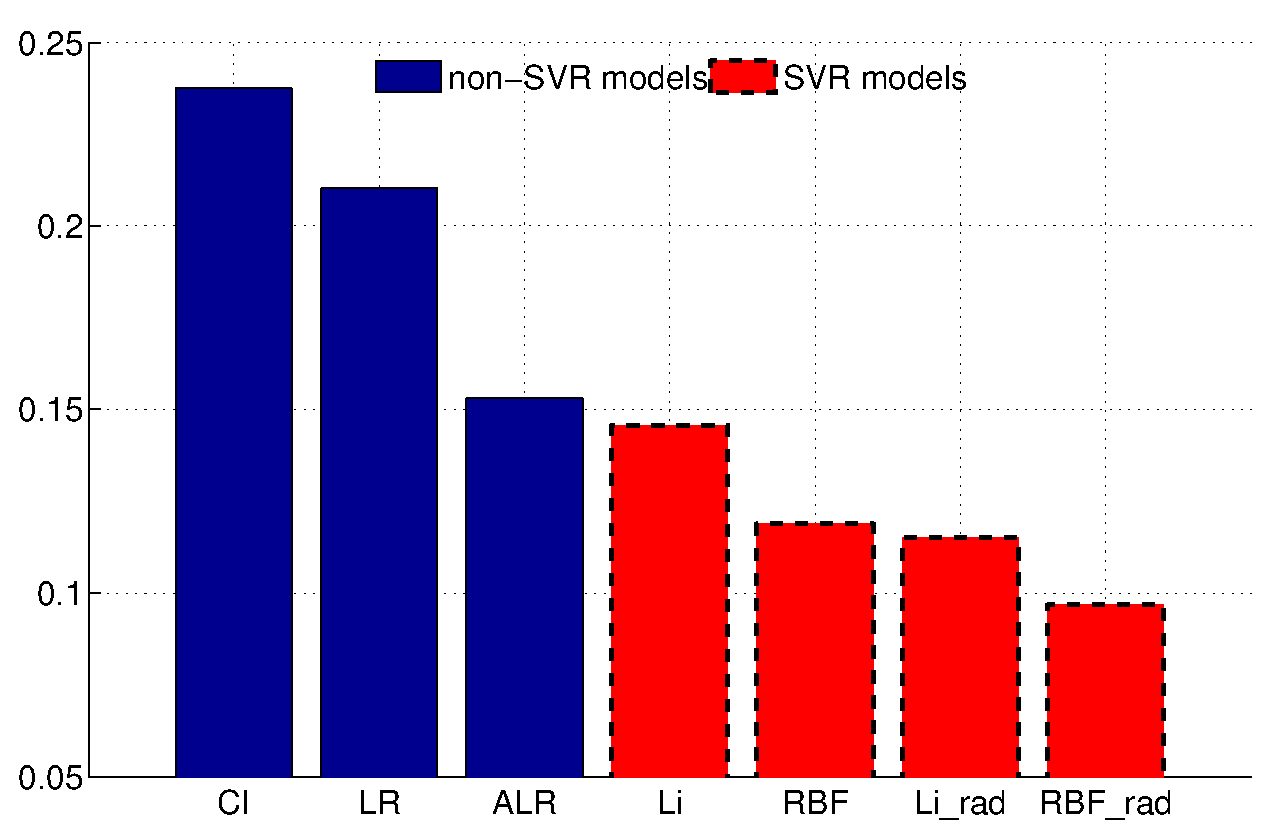
\includegraphics[width=3.2 in]{pics/modelsmae2}
\caption{MAE Plot of 5-fold cross validation. SVR models 
show less amounts of errors especially combined with previous radiation feature.}
\label{fig:modelsmae}
\end{figure}
 

\subsection{Model Comparison}
%non-SVR models contains CI and its linear extensions LR and ALR. For SVR models,
%we implement linear kernel ($SVR_{Li}$) and RBF kernel ($SVR-RBF$). With previous
%radiation feeding in as another evidence, SVR is extended to $SVR_{Li\_rad}$
%and $SVR_{RBF\_rad}$. The comparison of model performance is presented in
%figure \ref{fig:modelsmse} and figure \ref{fig:modelsmae}. 
We evaluate the irradiance modeling power using ground truth images.
As we described, we compare $CI$, $LR$ with single channel, $ALR$ which is $LR$ with 
multi-channel, $SVR_{Li}$ - SVR with multi-channel and linear kernel, $SVR_{RBF}$ - 
SVR with multi-channel and RBF kernel, $SVR_{Li\_rad}$ - $SVR_{Li}$ with the
previous timestamp radiation level, $SVR_{RBF\_rad}$ - $SVR_{RBF}$ 
with the previous timestamp radiation level.

First of all, Figure~\ref{fig:modelsmse} and \ref{fig:modelsmae} shows that CI
is worse than $LR$, which confirms that the weight coefficient learning help to learn better model.
Second, multi-channel data significantly decrease error rates ($LR$ vs $ALR$) and 
the previous timestamp radiation level is helpful to decrease error rates as well.
$SVR$ models are better than non-SVR models and non-linear kernel SVR models are even better.
% Since we might just go with MAE, I didn't add MSE and MAE comparison here.
Since $SVR_{RBF\_rad}$ showed the best performance, we will use it for 
motion estimation analysis.

\subsection{Motion Estimation Evaluation}
\label{subsec:MEEval}
To evaluate motion estimation in the context of radiation forecast applications, 
the motion estimation output of $HBM$ and $OF_{mean}$ are compared as the input to SVR models. 
We evaluated them from 0.5 to 5 hours of $SVR_{RBF\_rad}$ forecast results.
As a reference, we also add no motion estimation as our baseline (0 hour image as motion estimated image) 
and the original $OF$ which has no mean filter.  The MAE score is shown in
Figure \ref{fig:mesvrrbfrad}.
No motion estimation shows obviously the worst prediction quality but $HBM$ shows
slightly improvements over the baseline. Both $OF$ and $OF_{mean}$ shows significantly
better prediction quality and the mean filter is helpful across different
forecast time. It confirms that OF with mean filter is the best choice for satellite motion estimation
and we will use $OF_{mean}$ as our motion estimation method for next analysis.

% As the key procedure that influence accuracy of
% forecasting, motion tracking and image prediction are taken into evaluation by forecasting error from satellite model. In our experiment, two foreacast models are used as
% evaluation criteria. The first one is multi-channel SVR with RBF
% kernel($SVR-RBF$) which utilize non-linear relation to multi-channel value while the other
% one is multi-channel and previous radiation feature using RBF
% kernel($SVR_{RBF\_rad}$). The advantage of radiation feature is to minimize the
% noise from model itself. Mean Absolute Error(MAE) is used to indicate the
% forecast deviation from ground-truth irradiance.

% As introduced in Section \ref{sec:motionestimation}, we compared 2-frame
% Hierarchical Block Matching(HBM) with direct output of our Otical Flow Motion
% Estimation(OF) pipeline and final OF output after mean filter($OF_{mean}$).As
% reference of we also add no motion estimation to be the baseline. The
% comparison is shown in figure \ref{fig:mesvrrbf} and figure
% \ref{fig:mesvrrbfrad}. With targeting the hours' forecast to meet mid-term
% requirement, the experiment is designed to compare prediction output at 30 mintues,1 hour, 2 hour ,3 hour, 4
% hour and 5 hour. 

%\begin{figure}[h]
%\centering
%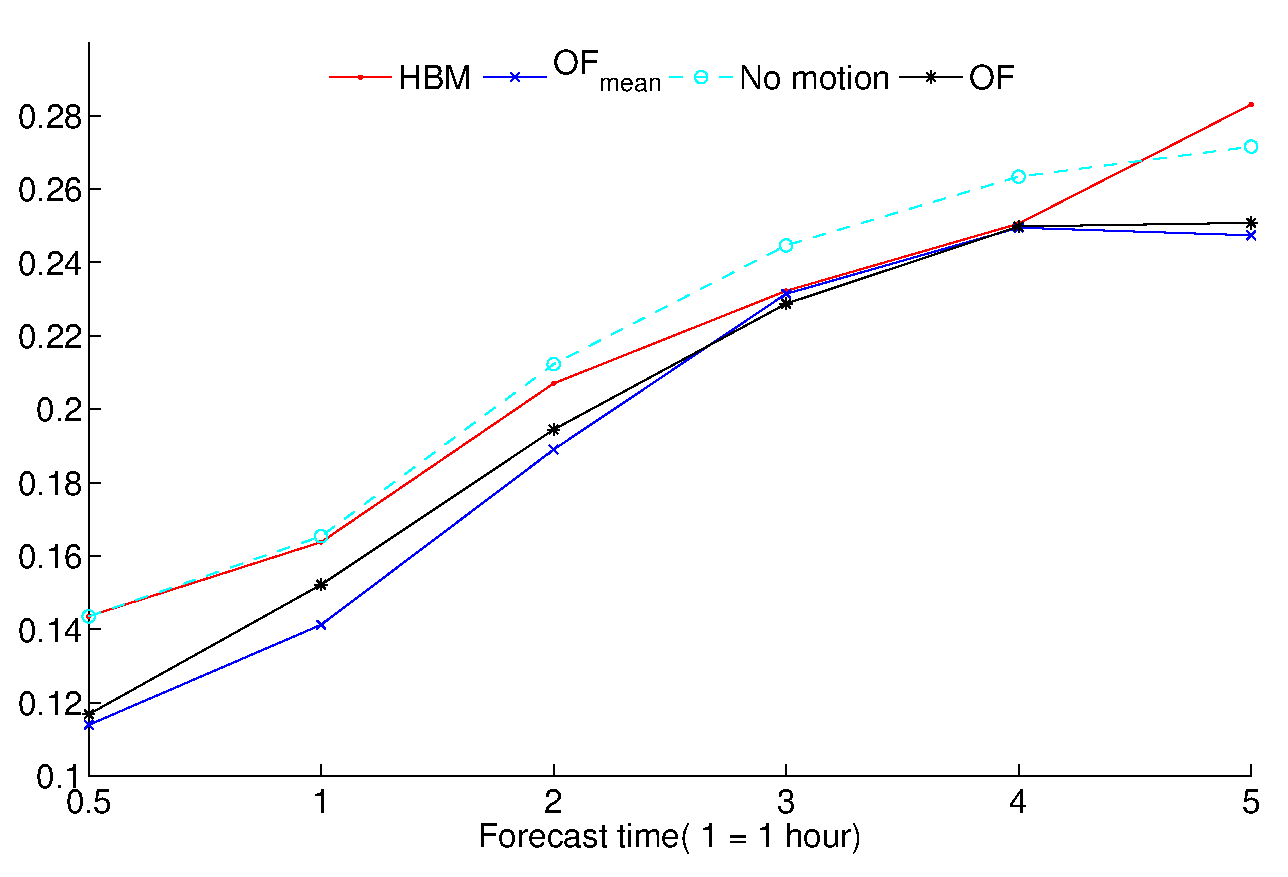
\includegraphics[width=3 in]{pics/SVRRBF}
%\label{fig:mesvrrbf}
%\caption{MAE of Motion Estimation using $SVR-RBF$ model}
%\end{figure}


\begin{figure}[tb]
\centering
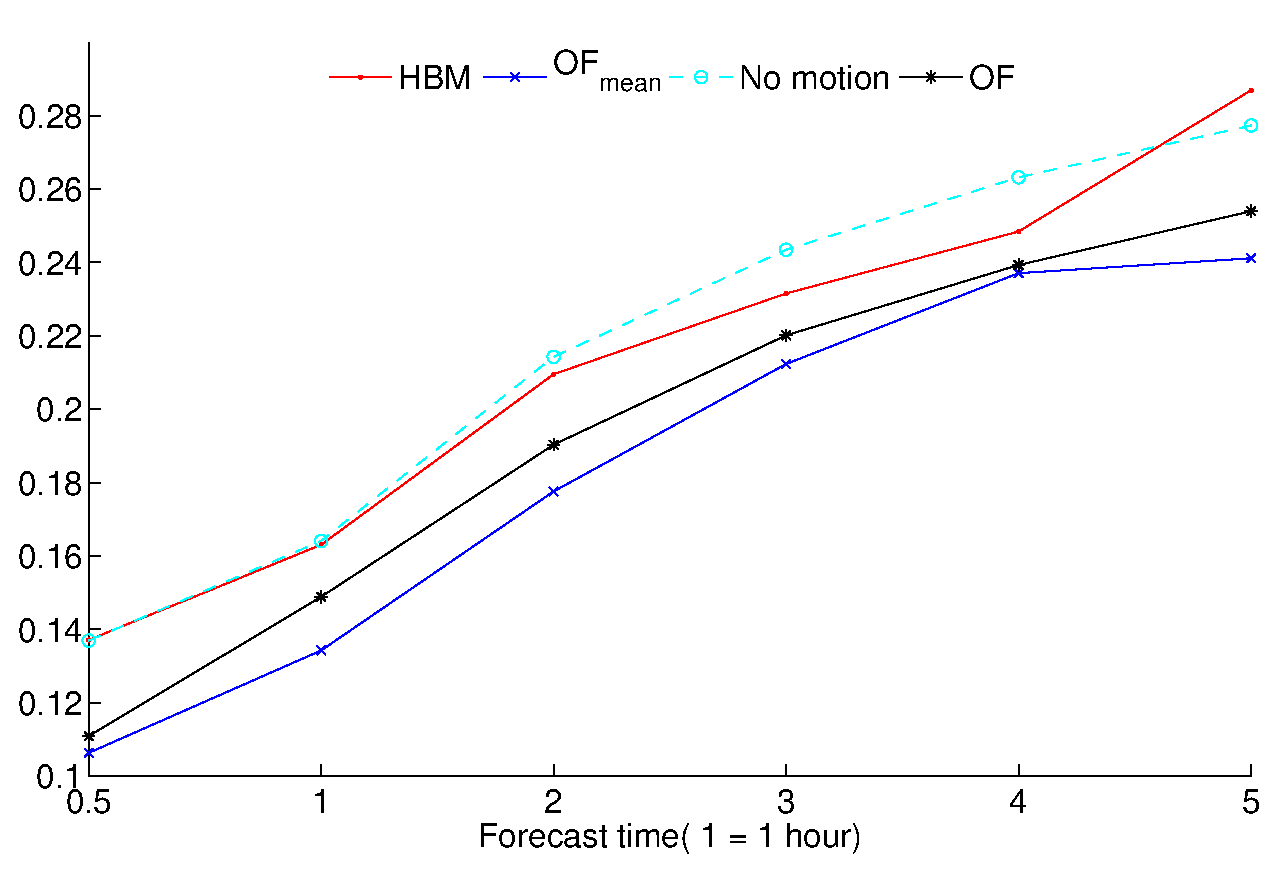
\includegraphics[width=3 in]{pics/SVRRBF_rad}
\caption{Motion estimation analysis using $SVR_{RBF\_rad}$ model (MAE). Both $OF_{mean}$
and $OF$ show less amounts of errors than HBM in 5 hours prediction}
\label{fig:mesvrrbfrad}
\end{figure}



\subsection{Irradiance Prediction Evaluation}
\label{subsec:forecast_e}
We analyze whether our model estimation results (without any forecast) are still hold or not. 
In other words, we investigate the noise effects of the motion estimation
on the irradiance prediction problem.
 
%figure \ref{fig:modelsmse_pre}
% only describes in terms of MAE
Since there are more errors due to motion estimation, $LR$ or $ALR$ shows even worse 
results than $CI$ (Figure \ref{fig:modelsmae_pre}) after four or five hours,
which is different from the model estimation results and expected as we discussed in Section \ref{sec:Models}.
However, the multi-channel of $ALR$ is still helpful to get much less error rates than $LR$.
In case of SVR, $SVR_{Li}$ is the worst among SVR models but with the additional radiation feature, 
it shows the best performance on or after three hours, which is also different from the model estimation results.
RBF kernel with the radiation feature is still the best results under two hours but as we have more and more errors 
from the motion estimation, it is not as robust as $SVR_{Li\_rad}$.
If we have an easy day for motion estimation, $SVR_{RBF\_rad}$ can be a good choice even after three hours
but if it is difficult to do good motion estimation and/or longer time forecasting, then $SVR_{Li\_rad}$ will be our choice.

%Similar to model performance comparison, MAE and MSE from ground measurement are used in terms of
%different forecast range. See details in figure \ref{fig:modelsmae_pre} and
%figure \ref{fig:modelsmse_pre}.

% Besides the purpose of comparison among models,
% forecasting output is also used for evaluation of motion estimation algorithms. As DFD value is a measurement of average error per image, MSE score of local scale(individual pixel) using SVR model is generated for performance comparison of motion estimation with time.
% The result is presented in Figure \ref{fig:mepred}. By using Optical Flow
% as motion estimation algorithm, the MSE and MAE score of 7 models is shown in
% Figure \ref{fig:modelsmse_pre} and Figure \ref{fig:modelsmae_pre}.

% \begin{figure}[h]
% \centering
% 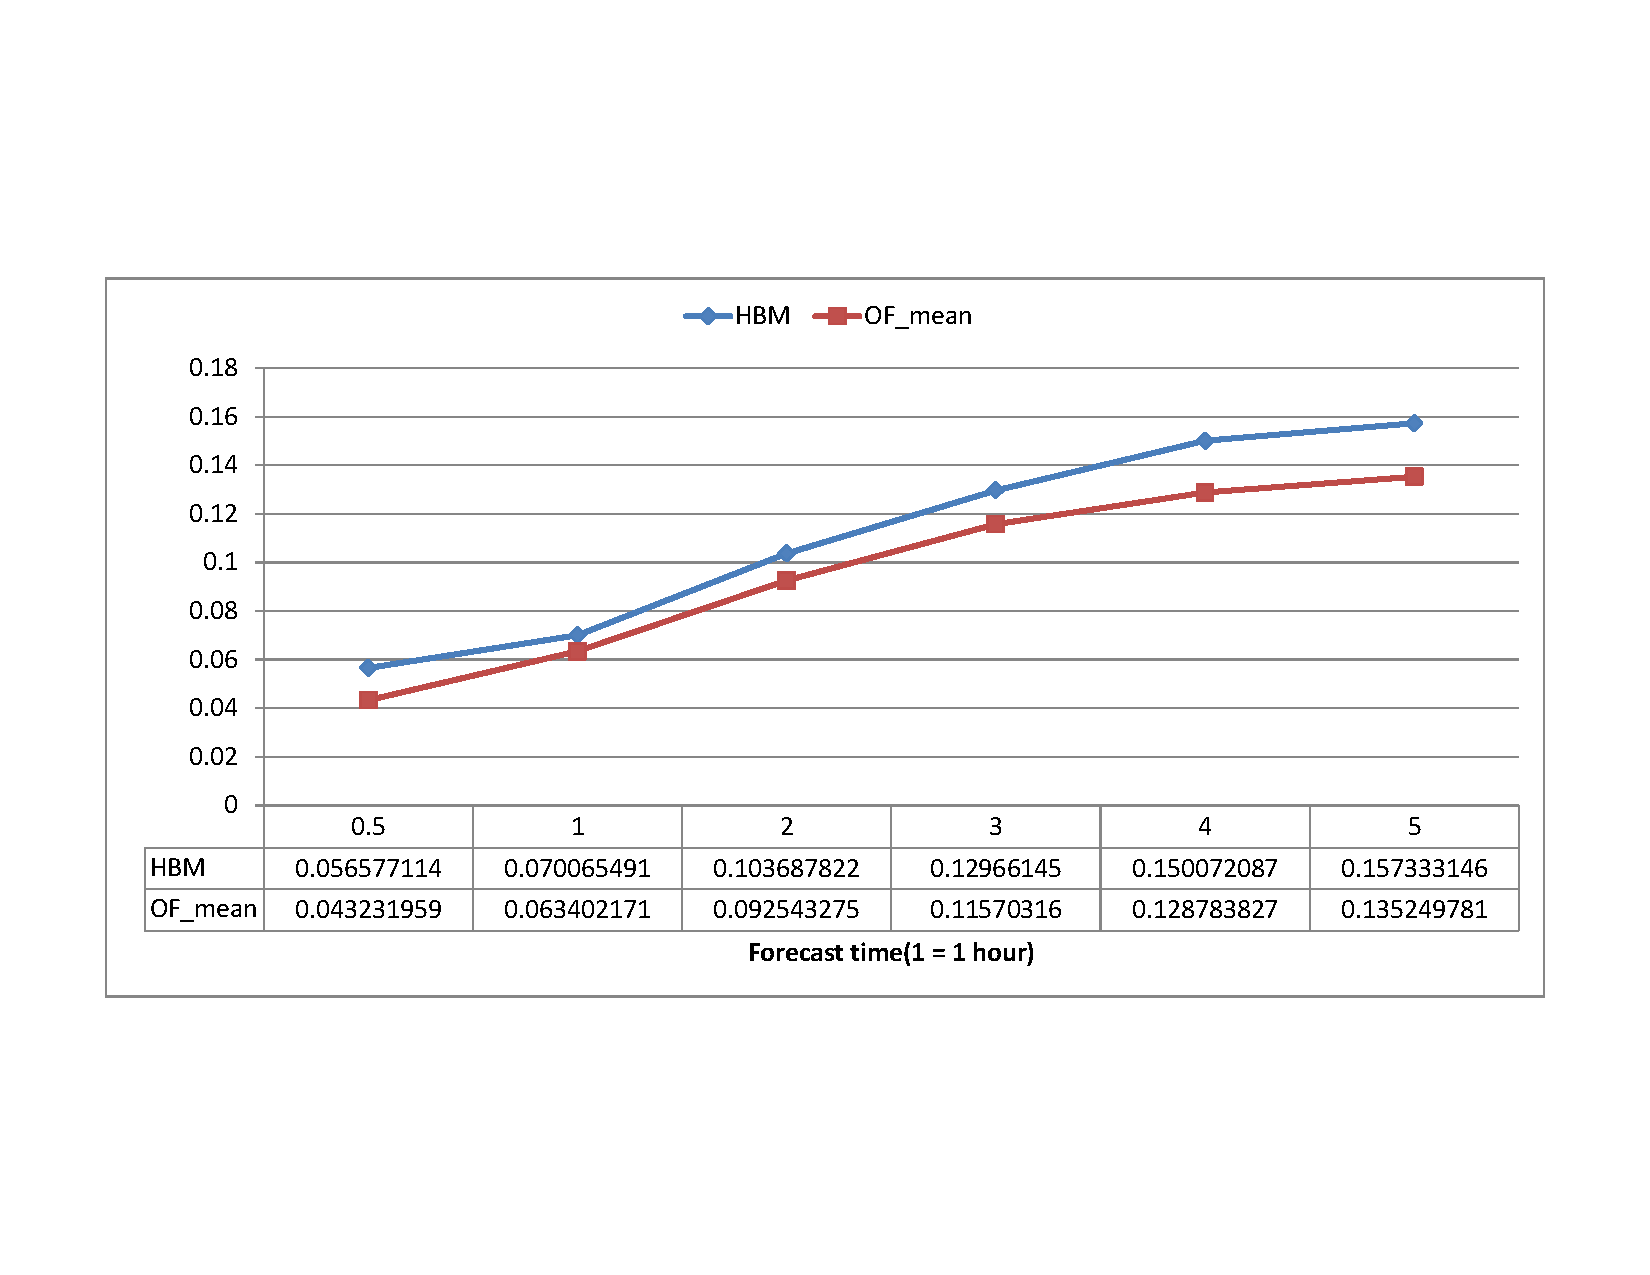
\includegraphics[width=2.5 in]{mepred}
% \label{fig:mepred}
% \caption{MSE score of Motion Estimation with $SVR_{RBF_rad} Forecasting$}
% \end{figure}

% \begin{figure}[tb]
% \centering
% 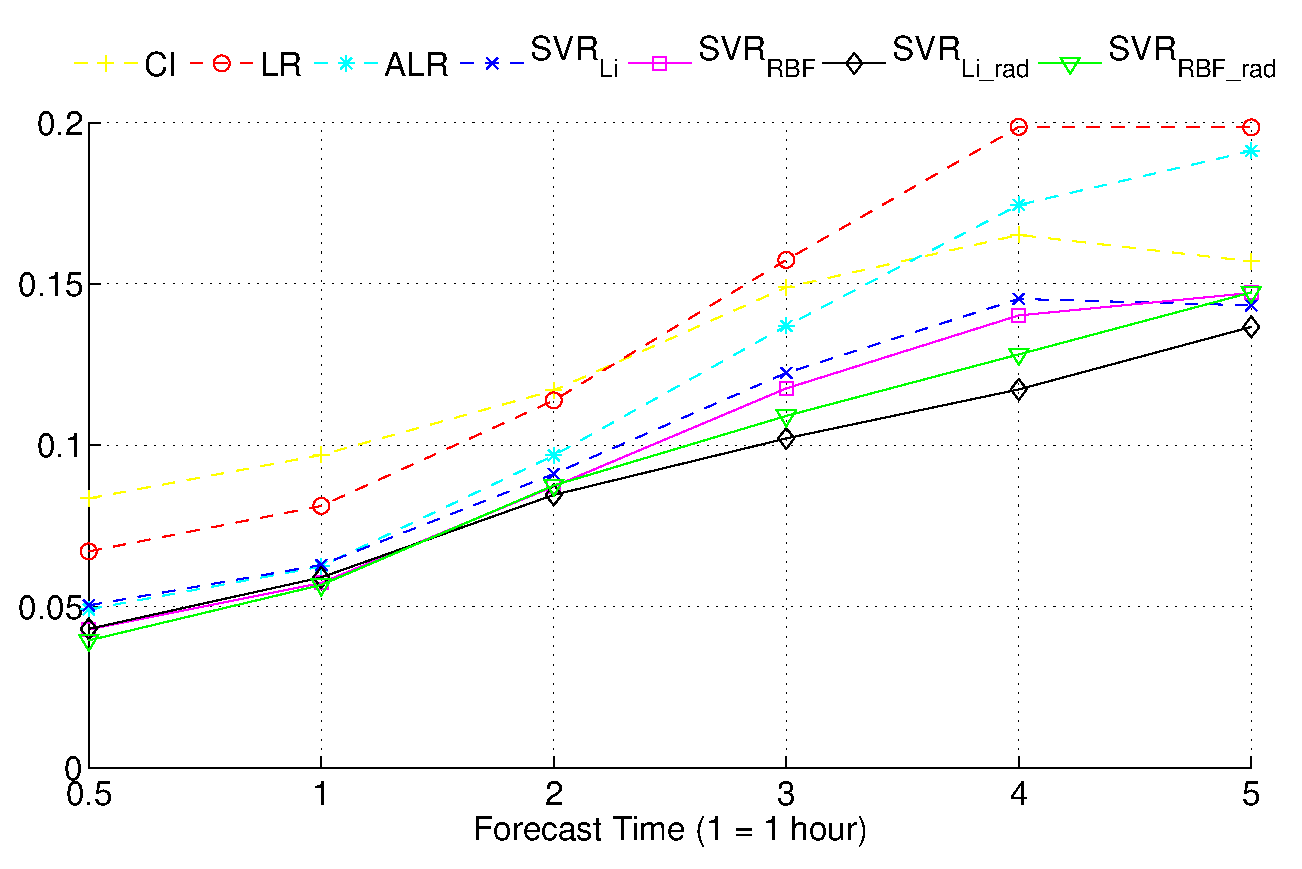
\includegraphics[width=3 in]{pics/predmse}
% \caption{MSE score of forecasting models}
% \label{fig:modelsmse_pre}
% \end{figure}


\begin{figure}[tb]
\centering
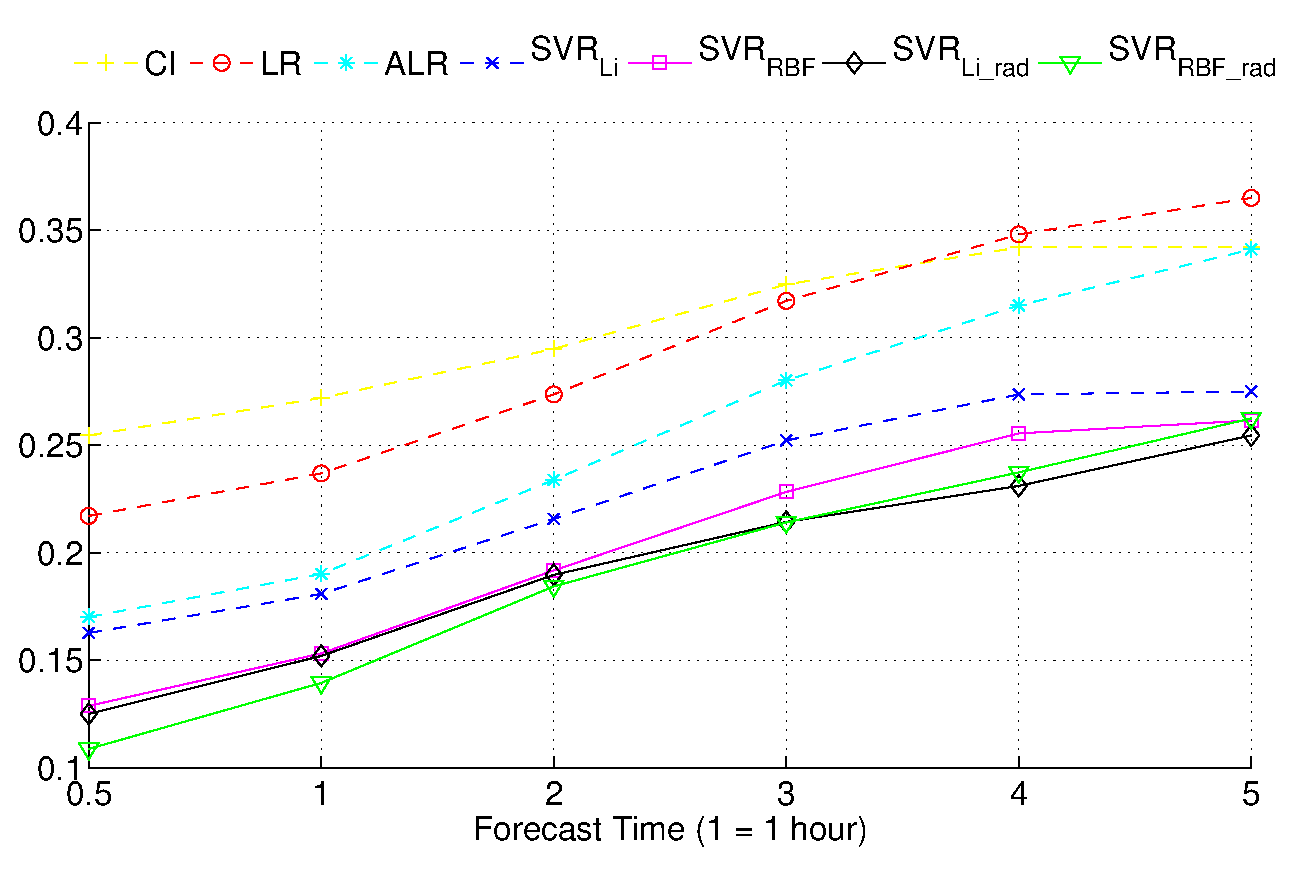
\includegraphics[width=3 in]{pics/predmae}
\caption{MAE score of 7 forecasting models using $OF_{mean}$.}
\label{fig:modelsmae_pre}
\end{figure}


\section{Conclusion} % 1) need better name 2) re-consider better place
% to put this section
\label{sec:conclusion}


In this paper, a new mid-term forecast system is developed with innovations on
both modeling and predicting aspect. To choose and compare the best satellite
models, we evaluated CI, LR, and SVR covering both linear and non-linear
approaches.
In cloud motion estimation, Optical Flow with mean filter shows the best performance
in both image-level analysis and forecasting evaluation. In hours'
forecasting, we find that SVR related models significantly improve the prediction accuracy
than non-SVR approaches. Although noise from cloud prediction increase
exponentially with time, the SVR with non-linear kernel and the previous radiation level 
still show the best results upto two hours
but the SVR with linear kernel and the previous radiation level could be a good candidate after three 
or more hour prediction ranges. The accuracy improvement is more than $50\%$ in 30 minutes 
prediction and $10\%$ in 5 hours prediction than the baseline satellite model.


\section{acknowledgment} 
\label{sec:acknowledgment}
This research is part of “A Public-Private-Academic Partnership
to Advance Solar Power Forecasting”. It is supported
in part by DOE grants DE-AC02-98CH10886.

\bibliography{document}
\bibliographystyle{IEEEtran}
%\bibliographystyle{plain}
%\bibliography{IEEEabrv,IEEEexample}



%\begin{thebibliography}{99}
%\begin{thebibliography}{1}
% \bibitem {Janjai09}
% Janjai S, Pankaew P, Laksanaboonsong J. \emph{A model for calculating hourly global
% solar radiation from satellite data in the tropics}, \hskip 1em plus 0.5em minus 0.4em\relax  Applied Energy 86.9 (2009): 1450-1457.
% 
% \bibitem {Janjai09}
% Janjai S, Pankaew P, Laksanaboonsong J. \emph{A model for calculating hourly global
% solar radiation from satellite data in the tropics}, \hskip 1em plus 0.5em minus 0.4em\relax  Applied Energy 86.9 (2009): 1450-1457.

%WB Rossow, LC Garder - Journal of Climate, 1993 – journals.ametsoc.org
%P Minnis, PW Heck, DF Young - Journal of the atmospheric …, 1993 -
% journals.ametsoc.org E Zaunick, J Levenhagen, K Janschek - 2011 – lib.physcon.ru
%RL Bankert, C Mitrescu, SD Miller… - Journal of applied …, 2009 –
% journals.ametsoc.org 
%[5]Janjai, S., P. Pankaew, and J. Laksanaboonsong. "A model for calculating
%hourly global solar radiation from satellite data in the tropics." Applied
% Energy 86.9 (2009): 1450-1457.
% [6] S¸ enkal O, Kuleli T. Estimation of solar radiation over Turkey using artificial
% neural network and satellite data. Applied Energy 2009;86(7e8):1222e8.
% [7]Zarzalejo LF, Ramírez L, Polo J. Artificial intelligence techniques applied to
% hourly global irradiance estimation from satellite-derived cloud index. Energy
% 2005;30:1685e97.
% [8] S¸ enkal O. Modeling of solar radiation using remote sensing and artificial neural network in Turkey. Energy 2010;35:4795e801.
% Cano, D. et al., 1986. A method for the determination of the global solar radiation from meteorological satellite data. Sol. Energy 37 (1), 31–39.
% Perez, R. et al., 2002. A new operational satellite-to-irradiance model—description and validation. Solar Energy 73 (5), 307–317.
% Schmetz, J. (1989): Towards a Surface Radiation Climatology: Retrieval of Downward Irradiances from Satellites. Atmos Res., 23, pp. 287-321
% Stuhlmann, R., Rieland, M., Raschke, E., 1989. An improvement of the IGMK model to derive total and diffuse solar radiation at the surface from satellite data. J. Appl. Meterol. 29, 586–603.
% Ineichen, P., Perez, R., 1999. Derivation of cloud index from geostationary satellites and application to the production of solar irradiance and daylight illuminance data. Theor. Appl. Climatol. 64, 119–130.
% Hammer, A., Heinemann, D., Hoyer, C., Kuhlemann, R.,Lorenz, E., Mueller, R., Beyer, H.G., 2003. Solar energy assessment using remote sensing technologies. Remote Sens. Environ. 86 (3), 423–432.
% Martins FR, Pereira EB, Abreu SL. Satellite-derived solar resource maps for Brazil under SWERA project. Solar Energy 2007;81:517–28.
% Janjai S, Laksanaboonsong J, Nunez M, Thongsathitya A. Development of a method generating operational solar radiation maps from satellite data for a tropical environment. Solar Energy 2005;78:739–51
% Pinker, R.T., Ewing, J.A., 1985. Modelling surface solar radiation: model formulation and validation. J. Appl. Meteorol. 24, 389–401.
% Zelenka, A., Perez, R., Seals, R., Renne, D., 1999. Effective accuracy of
% satellite-derived irradiance. Theor. Appl. Climatol. 62, 199–207
% Perez R, Ineichen P, Kmiecik M, Moore K, Renne D, George R. Producing
% satellite-derived irradiances in complex arid terrain. Solar Energy
% 2004;77:367–71.
% Zarzalejo, L.F.; Polo, J.; Martí L.; Ramí L.; Espinar, B. A new statistical approach for
% deriving global solar radiation from satellite images. Solar Energy 2009, 83, 480-484.
% Boser, Bernhard E.; Guyon, Isabelle M.; and Vapnik, Vladimir N.; A training algorithm for optimal margin classifiers. In Haussler, David (editor); 5th Annual ACM Workshop on COLT, pages 144–152, Pittsburgh, PA, 1992. ACM Press
%\end{thebibliography}

\end{document}
